\documentclass[10pt]{beamer}

% Include preamble files
% Package imports
\usepackage{media9}
\usepackage{amssymb,amsmath,amsthm,enumerate}
\usepackage[utf8]{inputenc}
\usepackage{array}
\usepackage[parfill]{parskip}
\usepackage{graphicx}
\usepackage{caption}
\usepackage{subcaption}
\usepackage{bm}
\usepackage{amsfonts,amscd}
\usepackage[]{units}
\usepackage{listings}
\usepackage{multicol}
\usepackage{multirow}
\usepackage{tcolorbox}
\usepackage{physics}
\usepackage{algorithm2e}
\usepackage{lastpage}
\usepackage{pifont}
\usepackage{animate}
\usepackage{ifthen}
\usepackage{hyperref}
\usepackage{pgffor}
\usepackage[margin=1in]{geometry}
\usepackage[acronym]{glossaries}
\usepackage[style=ieee]{biblatex}
% \lstset{basicstyle=\ttfamily\small} % optional settings

\lstset{
  basicstyle=\ttfamily\small,
  keywordstyle=\color{blue},
  commentstyle=\color{gray},
  breaklines=true
}

% Enable colored hyperlinks
\hypersetup{colorlinks=true}

% Numbered captions of tables, pictures, etc.
\setbeamertemplate{caption}[numbered]

% Bibliography settings
\setbeamertemplate{bibliography item}{\insertbiblabel}
\addbibresource{references.bib} 

% --- Customization for enumerated ToC ---
% Set templates for sections and subsections in the ToC to be numbered
% Even vertical spacing and top alignment for ToC items, with top/bottom padding
\setbeamertemplate{section in toc}[sections numbered]
\setbeamertemplate{toc item}{\vspace{0.7em}} % Adjust spacing as needed
\addtobeamertemplate{frametitle}{}{\vspace*{-\baselineskip}} % Remove extra space above ToC
\setbeamertemplate{toc}{%
  \vbox{%
    \vspace*{1.5em} % Top padding
    \insertbeamertoc
    \vspace*{1.5em} % Bottom padding
  }
}
% Indent subsections in ToC by 4 spaces and put each on a new line
\setbeamertemplate{subsection in toc}{%
  \par\hspace*{1em}\inserttocsubsectionnumber.\;\inserttocsubsection%
}
% --- End Customization ---

% Custom commands
\newcommand{\R}{\mathbb{R}}
\renewcommand{\thealgocf}{}

% Crossmarks & checkmarks
\newcommand{\cmark}{\ding{51}}
\newcommand{\xmark}{\ding{55}}

% Colored emphasis
\newcommand{\empy}[1]{{\color{darkorange}\emph{#1}}}
\newcommand{\empr}[1]{{\color{blue}\emph{#1}}}

% A command to fetch an image via curl if it doesn't yet exist
\newcommand{\fetchimage}[2]{%
  \IfFileExists{#1}{}{%
    \immediate\write18{curl -sL "#2" -o "#1"}%
  }%
}

% Robust macro to fetch and convert web image to PNG for LaTeX
% Requires shell-escape, curl, and ImageMagick (convert)
\newcommand{\fetchconvertimageonly}[2]{%
  \IfFileExists{#2}{}{%
    \immediate\write18{curl -sL "#1" -o "temp_image_download"}%
    \immediate\write18{convert temp_image_download "#2"}%
    \immediate\write18{rm -f temp_image_download}%
  }%
}

% Robust macro to fetch and convert web image to PNG for LaTeX
% Requires shell-escape, curl, and ImageMagick (convert)
\newcommand{\fetchconvertimage}[3]{%
  \IfFileExists{#2}{}{%
    \immediate\write18{curl -sL "#1" -o "temp_image_download"}%
    \immediate\write18{convert temp_image_download "#2"}%
    \immediate\write18{rm -f temp_image_download}%
  }%
  \includegraphics[#3]{#2}%
}

% Adaptive macro to convert a GIF into frames and animate it
% Usage: \includeGIF{your.gif}{basename}{width}{fps}
\newcommand{\includeGIF}[4]{%
  % % Frame path prefix
  % \def\gifpath{gif_frames}%
  % \def\frameprefix{\gifpath/#2_}%

  % % If frames don't exist, extract them
  % \IfFileExists{\frameprefix000.png}{}{%
  %   \immediate\write18{mkdir -p \gifpath}%
  %   \immediate\write18{convert "#1" "\frameprefix%03d.png"}%
  %   % Count frames using identify
  %   \immediate\write18{identify -format \%n "#1" > \gifpath/#2_framecount.txt}%
  % }%

  % % Read frame count
  % \newread\framecountfile%
  % \openin\framecountfile=\gifpath/#2_framecount.txt%
  % \read\framecountfile to \totalframes%
  % \closein\framecountfile%

  % % Decrement for zero-based indexing (e.g., 10 frames = 000 to 009)
  % \newcount\lastframe
  % \lastframe=\totalframes
  % \advance\lastframe by -1

  % % Pad last frame (e.g., 9 becomes 009)
  % \edef\lastframepad{\ifnum\lastframe<10 00\the\lastframe\else\ifnum\lastframe<100 0\the\lastframe\else\the\lastframe\fi\fi}%

  % % Animate using detected frame range
  % \animategraphics[loop,controls,width=#3]{#4}{\frameprefix}{000}{\lastframepad}%

  \begingroup
  \def\giffile{#1}%
  \def\basename{#2}%
  \def\widthval{#3}%
  \def\fpsval{#4}%
  \def\gifpath{gif_frames}%
  \def\frameprefix{\gifpath/\basename\_}%

  \IfFileExists{\frameprefix000.png}{}{%
    \immediate\write18{mkdir -p \gifpath}%
    \immediate\write18{convert "\giffile" "\frameprefix%03d.png"}%
    \immediate\write18{identify -format %%n "\giffile" > "\gifpath/\basename\_framecount.txt"}%
  }%

  \newread\framecountfile%
  \openin\framecountfile=\gifpath/\basename\_framecount.txt%
  \read\framecountfile to \totalframes%
  \closein\framecountfile%

  \newcount\lastframe
  \lastframe=\totalframes
  \advance\lastframe by -1

  % Format last frame number as zero-padded (e.g., 9 -> 009)
  \def\lastframepad{\ifnum\lastframe<10 00\the\lastframe\else%
    \ifnum\lastframe<100 0\the\lastframe\else%
    \the\lastframe\fi\fi}%

  \animategraphics[loop,controls,width=\widthval]{\fpsval}{\frameprefix}{000}{\lastframepad}%
  \endgroup
}


% Example box
\newcommand{\examplebox}[2]{
\begin{tcolorbox}[colframe=darkcardinal,colback=boxgray,title=#1]
#2
\end{tcolorbox}}

% Theorem environments
\theoremstyle{remark}
\newtheorem*{remark}{Remark}
\theoremstyle{definition}

% Glossary entries
\newacronym{ML}{ML}{machine learning} 
% Beamer settings
\usetheme{Stanford} 
\def \i  {\item}
\def \ai {\item[] \quad \arrowbullet}
\newcommand \si[1]{\item[] \quad \bulletcolor{#1}}
\def \wi {\item[] \quad $\ \phantom{\Rightarrow}\ $}
\def \bi {\begin{itemize}\item}
\def \ei {\end{itemize}}
\def \be {\begin{equation*}}
\def \ee {\end{equation*}}
\def \bie {$\displaystyle{}
\def \eie {{\ }$}}
\def \bsie {\small$\displaystyle{}
\def \esie {{\ }$}\normalsize\selectfont}
\def \bse {\small\begin{equation*}}
\def \ese {\end{equation*}\normalsize}
\def \bfe {\footnotesize\begin{equation*}}
\def \efe {\end{equation*}\normalsize}
\renewcommand \le[1] {\\ \medskip \lefteqn{\hspace{1cm}#1} \medskip}
\def \bex {\begin{example}}
\def \eex {\end{example}}
\def \bfig {\begin{figure}}
\def \efig {\end{figure}}
\def \btheo {\begin{theorem}}
\def \etheo {\end{theorem}}
\def \bc {\begin{columns}}
\def \ec {\end{columns}}
\def \btab {\begin{tabbing}}
\def \etab {\end{tabbing}\svneg\svneg}
\newcommand \col[1]{\column{#1\linewidth}}
\def\vneg  {\vspace{-5mm}}
\def\lvneg {\vspace{-10mm}}
\def\svneg {\vspace{-2mm}}
\def\tvneg {\vspace{-1mm}}
\def\vpos  {\vspace{5mm}}
\def\lvpos {\vspace{10mm}}
\def\svpos {\vspace{2mm}}
\def\tvpos {\vspace{1mm}}
\def\hneg  {\hspace{-5mm}}
\def\lhneg {\hspace{-10mm}}
\def\shneg {\hspace{-2mm}}
\def\thneg {\hspace{-1mm}}
\def\hpos  {\hspace{5mm}}
\def\lhpos {\hspace{10mm}}
\def\shpos {\hspace{2mm}}

\logo{
\includegraphics[height=0.4in]{style_files/kaust_academy_logo.png}}

% Commands to relax beamer and subfig conflicts
\makeatletter
\let\@@magyar@captionfix\relax
\makeatother

% Set itemize styles
\setbeamertemplate{itemize items}[default]
\setbeamertemplate{itemize subitem}[circle] 

\title[Convolutional Neural Network]{Convolutional Neural Network (Recap)}

\begin{document}

% Include sections
% Title page
\author[KAUST Academy]{
    \begin{tabular}{c} 
    \Large
    Naeemullah Khan\\
    \footnotesize \href{mailto:naeemullah.khan@kaust.edu.sa}{naeemullah.khan@kaust.edu.sa}
    \end{tabular}
    \vspace{-4ex}
}

\institute{
    \vskip 20pt
    \begin{figure}
        \centering
        \begin{subfigure}[t]{0.5\textwidth}
            \centering
            
\includegraphics[height=0.5in]{style_files/kaust_logo.png}
        \end{subfigure}
    \end{figure}
    \vskip 20pt
    KAUST Academy \\
    King Abdullah University of Science and Technology\\
    \vskip 3pt
}

\date{\today}

\begin{noheadline}
\begin{frame}\maketitle\end{frame}
\end{noheadline}

% Table of Contents
\begin{frame}[allowframebreaks]{Table of Contents}
\begin{enumerate}
    \item Challenges
    \item Intersection over Union (IoU)
    \item Single Object Detection
    \item Multiple Objects & Sliding Window
    \item Region Proposal Networks (RPN)
    \item R-CNN
    \item Fast R-CNN
    \item Faster R-CNN
    \item YOLO 
    \item Summary
\end{enumerate}
\end{frame}
\begin{frame}[allowframebreaks]{\textcolor{green}{$\Rightarrow$} Learning Outcomes}
    By the end of this session, you will be able to:
    \begin{itemize}
        \item Explain what a VAE is and why we use it
        \item Describe how VAEs create and use hidden (latent) spaces
        \item Understand how VAEs learn from data
        \item Understand the ELBO and its role
        \item See how we train VAEs using special tricks
        \item Recognize different types of VAEs and some common challenges
    \end{itemize}
\end{frame}
\begin{frame}{}
    \LARGE GANs: \textbf{Definition and Core Components}
\end{frame}

\begin{frame}{Definition and Core Components}
\begin{itemize}
    \item Let $S_1 = D = \{x \sim p_{\text{data}}\}$ and $S_2 = \{x \sim p_\theta\}$.
    \item \textbf{Idea}: Train the generative model to minimize a two-sample test objective between $S_1$ and $S_2$, i.e., the generator.
    \item<2-> \textbf{Question}: How do we obtain a two-sample test objective?
    \item<3-> \textbf{Another Idea}: Train another neural network to discriminate between the two samples, i.e., the discriminator.
    \item<4-> And Voila! That's how we arrive at a GAN. The remaining step is to define the training method.
\end{itemize}
\end{frame}

\begin{frame}[allowframebreaks]{GANs: Definition and Core Components}
\begin{figure}
    \centering
    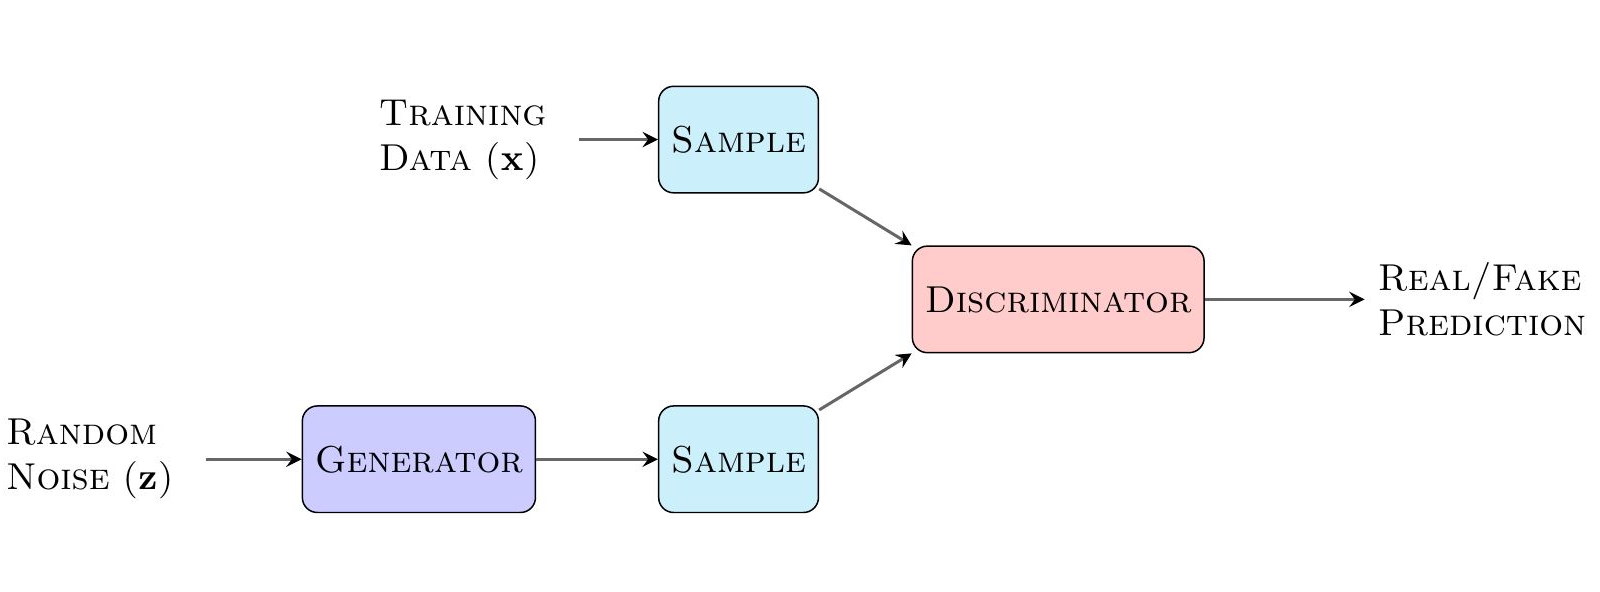
\includegraphics[height=0.7\textheight, width=\textwidth, keepaspectratio]{images/gan/gan_1.png}
    \caption*{A GAN model diagram\footnote{https://github.com/JamesAllingham/LaTeX-TikZ-Diagrams}}
\end{figure}

\framebreak

\begin{itemize}
    \item Generative Adversarial Networks were introduced by Ian Goodfellow et al. (2014).
    \item The idea behind GANs is to train two networks jointly:
    \begin{itemize}
        \item A \textbf{discriminator (D)} to classify samples as “real” or “fake”.
        \item A \textbf{generator (G)} to map a simple fixed distribution to samples that fool \textbf{D}.
    \end{itemize}
    \item The approach is \textbf{adversarial} since the two networks have opposing objectives.
\end{itemize}

\framebreak
\begin{figure}
    \centering
    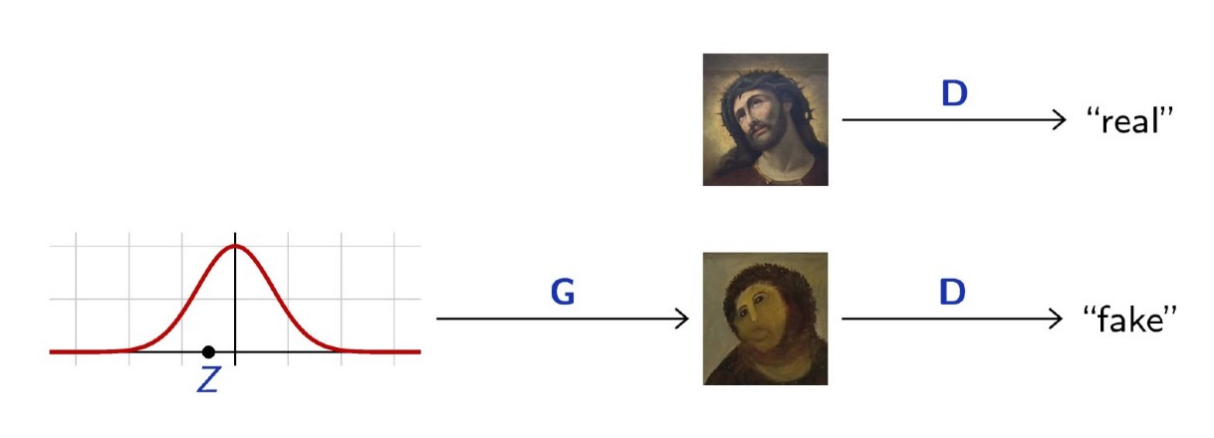
\includegraphics[height=0.7\textheight, width=\textwidth, keepaspectratio]{images/gan/gan_2.png}
    \caption*{The generator transforms a simple distribution into samples resembling real data. The discriminator distinguishes between real and fake samples.}
\end{figure}
\end{frame}
\subsection{Convolutional Layer}
\begin{frame}{}
    \LARGE CNN Layer: \textbf{Convolutional Layer}
\end{frame}
\begin{frame}[fragile]{Convolutional Layer}
\begin{block}{Operation:}
    \begin{itemize}
        \item Element‑wise multiply filter with image patch and sum → feature map.
    \end{itemize}
\end{block}

\begin{block}{Hyperparameters:}
    \begin{itemize}
        \item kernel size
        \item number of filters
        \item stride
        \item padding
    \end{itemize}
\end{block}

\begin{lstlisting}[language=Python, caption={Code snippet (PyTorch)}, basicstyle=\ttfamily\footnotesize]
import torch.nn as nn

conv = nn.Conv2d(in_channels=3, out_channels=16, kernel_size=3, stride=1, padding=1)

output = conv(input_tensor)  # input_tensor: [batch_size, 3, H, W]
\end{lstlisting}
\end{frame}  

\begin{frame}{CNN - Convolutional Layer}
    \begin{figure}
    \centering
    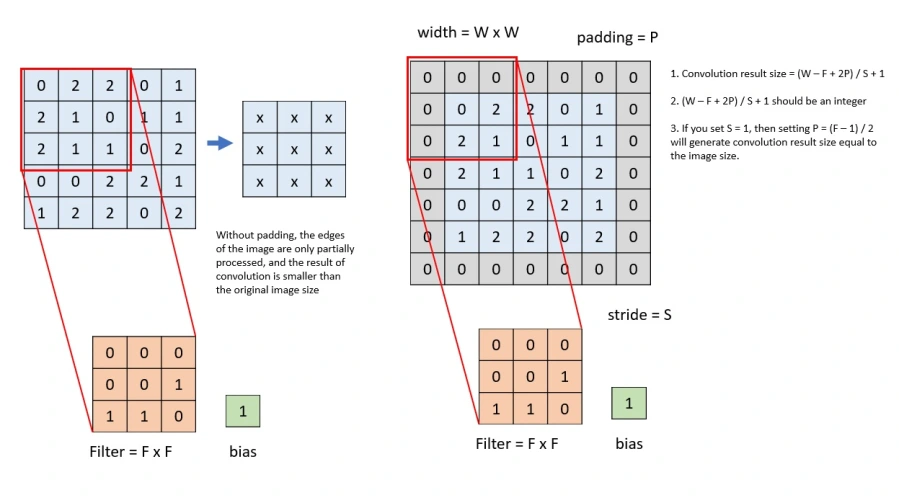
\includegraphics[width=0.95\textwidth,height=0.95\textheight,keepaspectratio]{images/cnn/convolutional-layer.png}
    \end{figure}

    \href{https://cs231n.github.io/convolutional-networks/}{Interactive demo: cs231n.github.io/convolutional-networks}
\end{frame}

% \begin{frame}{Quick Exercise (5 mins)}
%     \begin{block}{Let’s find out what this can give us:}
%         \begin{itemize}
%             \item Padding = 0
%             \item Stride = 1
%         \end{itemize}
%     \end{block}
%     \begin{figure}
%     \centering
%     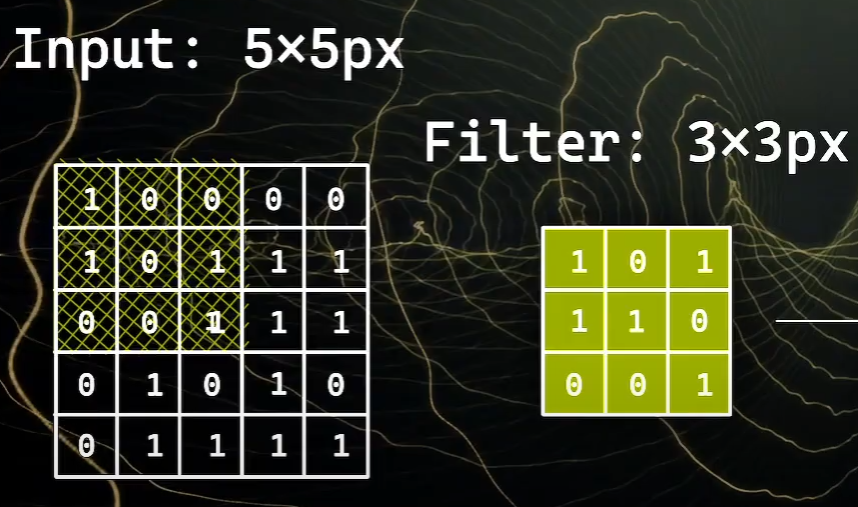
\includegraphics[width=0.7\textwidth,height=0.7\textheight,keepaspectratio]{images/cnn/cnn-exercise-1.png}
%     \end{figure}

%     Note: Once you traverse entire image/matrix it will give you a matrix calls Feature Map or Activation Map.
% \end{frame}
\begin{frame}[fragile]{CNN - Activation Functions}
\begin{block}{Role:}
    \begin{itemize}
        \item Introduce non‑linearity so multiple conv layers can learn complex mappings.
    \end{itemize}
\end{block}

\begin{block}{Common:}
    \begin{itemize}
        \item ReLU (Rectified Linear Unit)
        \item Leaky ReLU
        \item Sigmoid
        \item Tanh
    \end{itemize}
\end{block}

\begin{lstlisting}[language=Python, caption={Code snippet (PyTorch)}, basicstyle=\ttfamily\footnotesize]
import torch.nn.functional as F

x = conv(input_tensor)
x = F.relu(x)              # ReLU
x = F.leaky_relu(x, 0.1)   # Leaky ReLU
\end{lstlisting}
\end{frame}  

\begin{frame}{CNN - Activation Functions}
    \begin{figure}
    \centering
    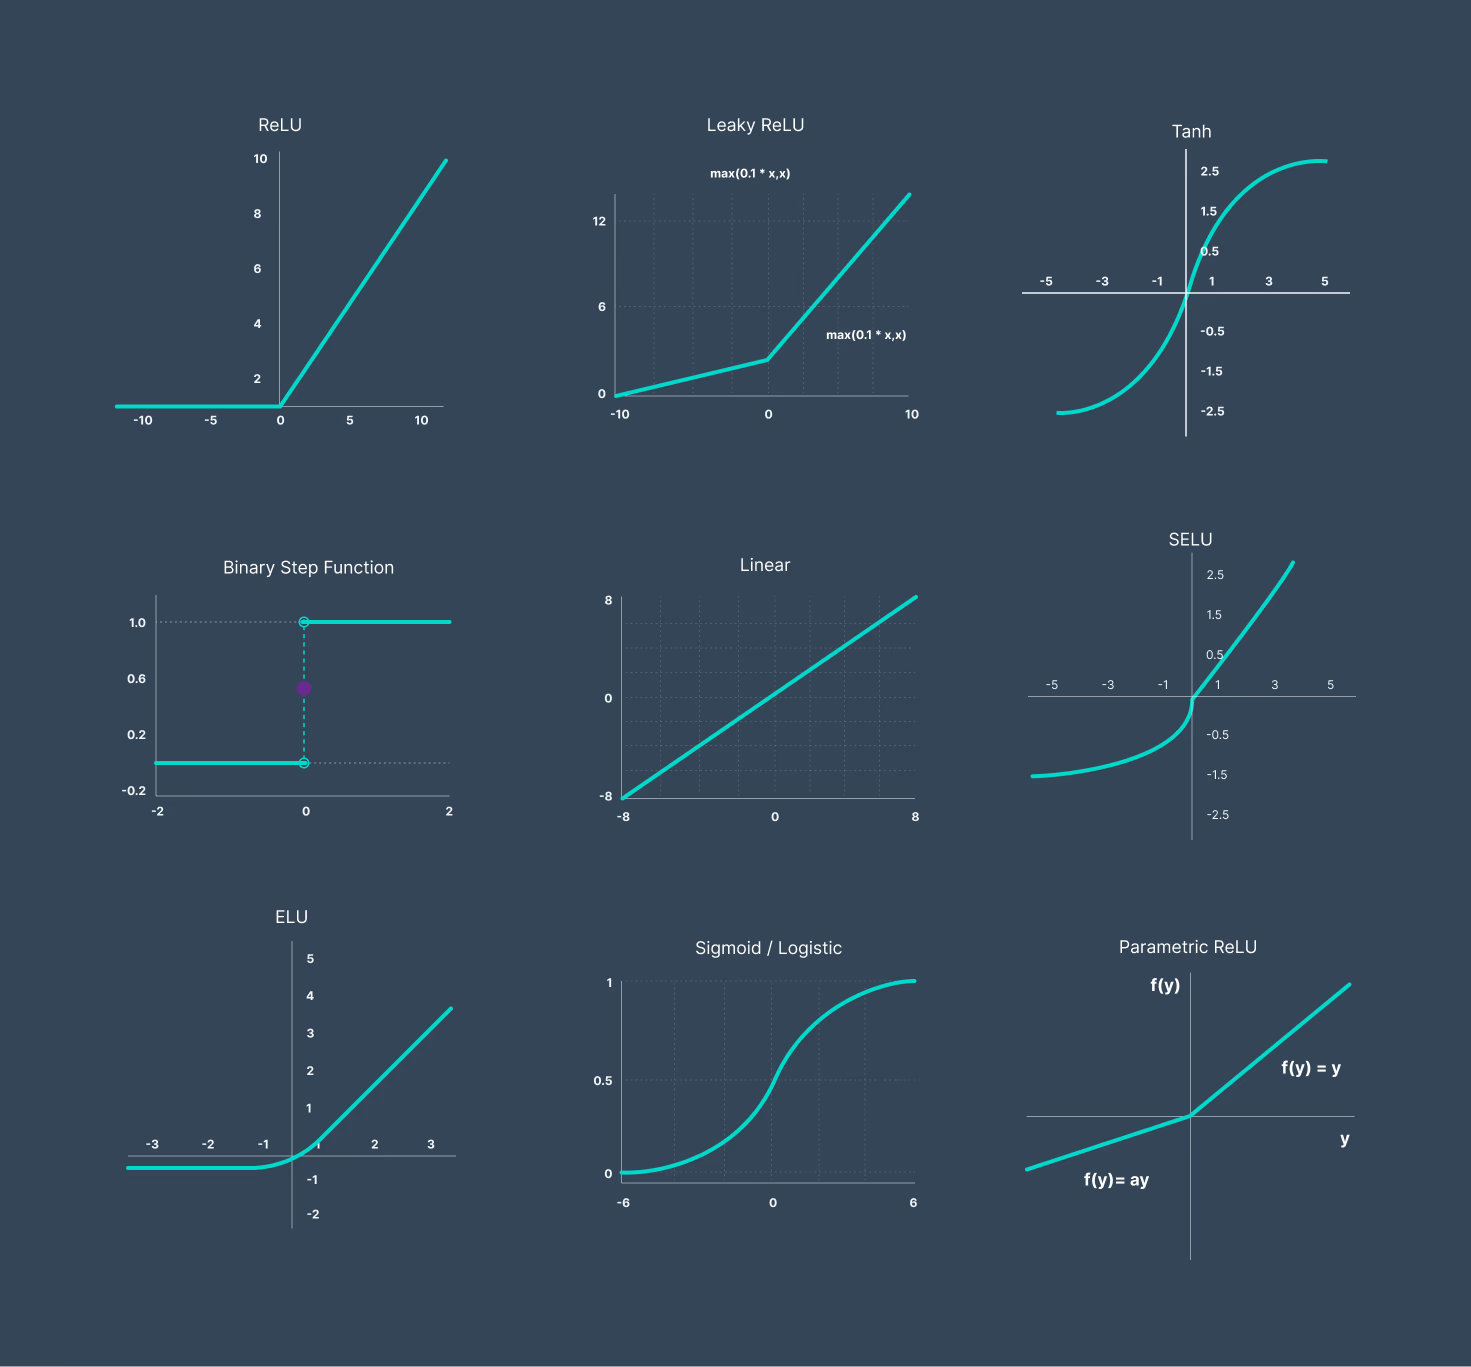
\includegraphics[width=0.95\textwidth,height=0.95\textheight,keepaspectratio]{images/cnn/activation-functions.png}
    \end{figure}
\end{frame}
\subsection{Pooling Layers}
\begin{frame}{}
    \LARGE CNN Layer: \textbf{Pooling Layers}
\end{frame}

\begin{frame}[allowframebreaks]{Pooling}

\begin{itemize}
    \item Compute mean or max over small windows to reduce resolution
\end{itemize}


\begin{figure}
\centering
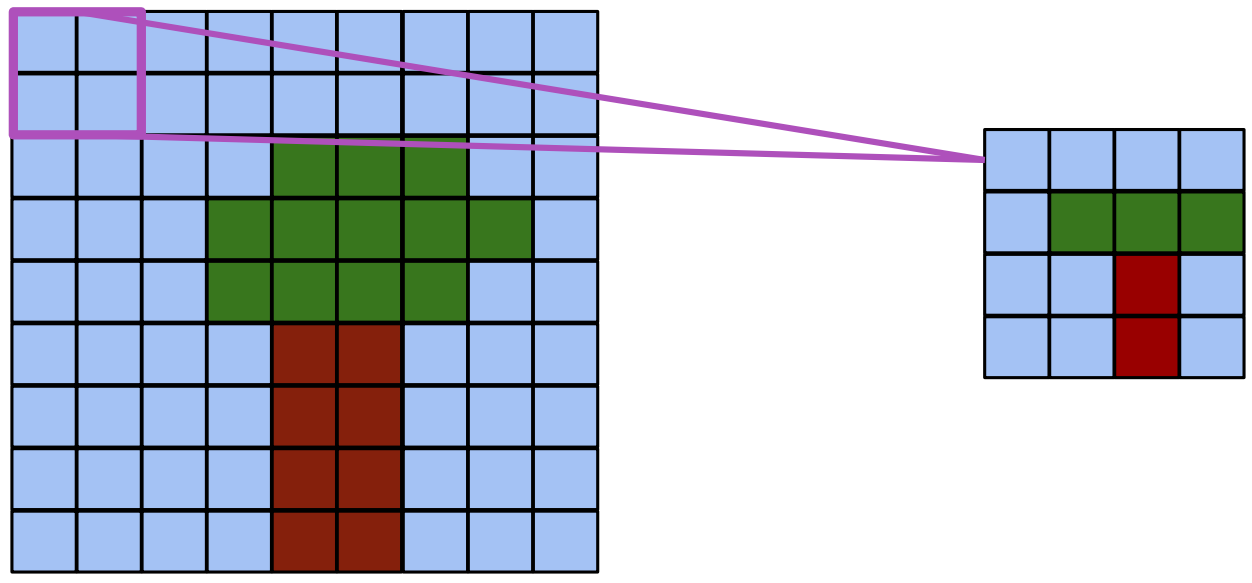
\includegraphics[width=1.0\textwidth,height=0.8\textheight,keepaspectratio]{images/cnn/pool_1.png}
\end{figure}

\framebreak

\begin{figure}
\centering
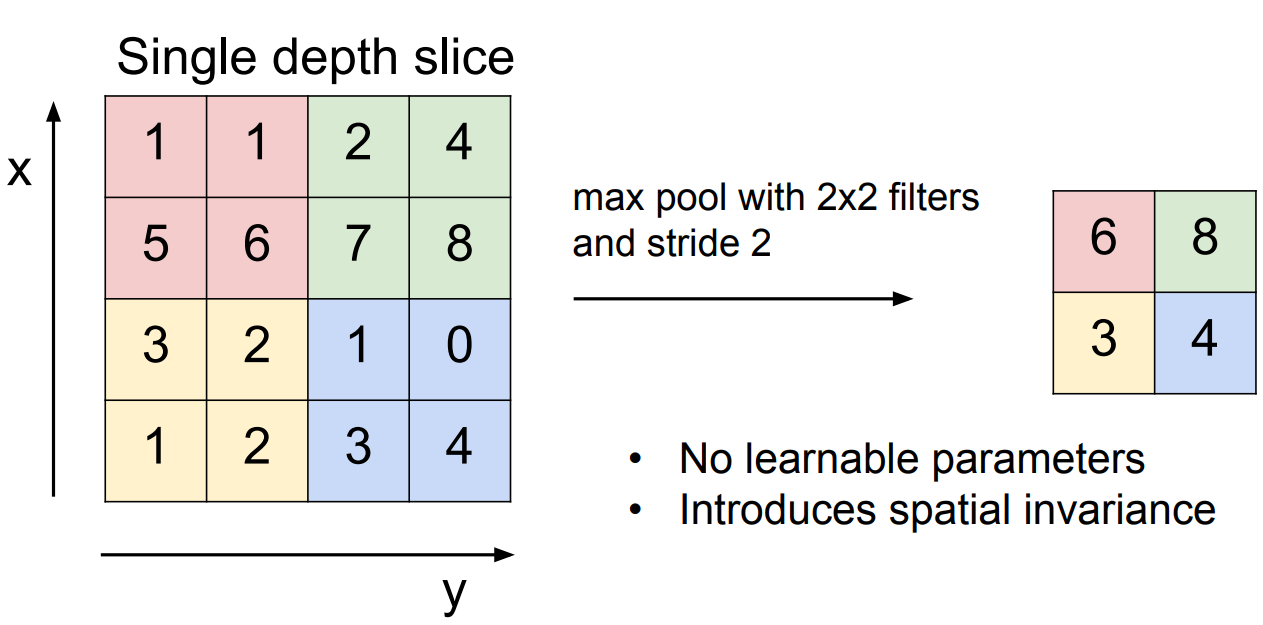
\includegraphics[width=1.0\textwidth,height=0.8\textheight,keepaspectratio]{images/cnn/pool_2.png}
\end{figure}
    
\end{frame}

\begin{frame}[fragile]{Pooling Layers}
\begin{block}{Purpose:}
    \begin{itemize}
        \item Downsample feature maps, reduce spatial dims and parameters, add invariance.
    \end{itemize}
\end{block}

\begin{block}{Types:}
    \begin{itemize}
        \item Max Pooling
        \item Average Pooling
        \item Global Average Pooling
        \item Global Max Pooling
    \end{itemize}
\end{block}

\begin{lstlisting}[language=Python, caption={Code snippet (PyTorch)}, basicstyle=\ttfamily\footnotesize]
import torch.nn as nn

pool = nn.MaxPool2d(kernel_size=2, stride=2)
pooled = pool(x)  # halves H and W
\end{lstlisting}
\end{frame}  

\begin{frame}[allowframebreaks]{Pooling Layers}
    \begin{figure}
    \centering
    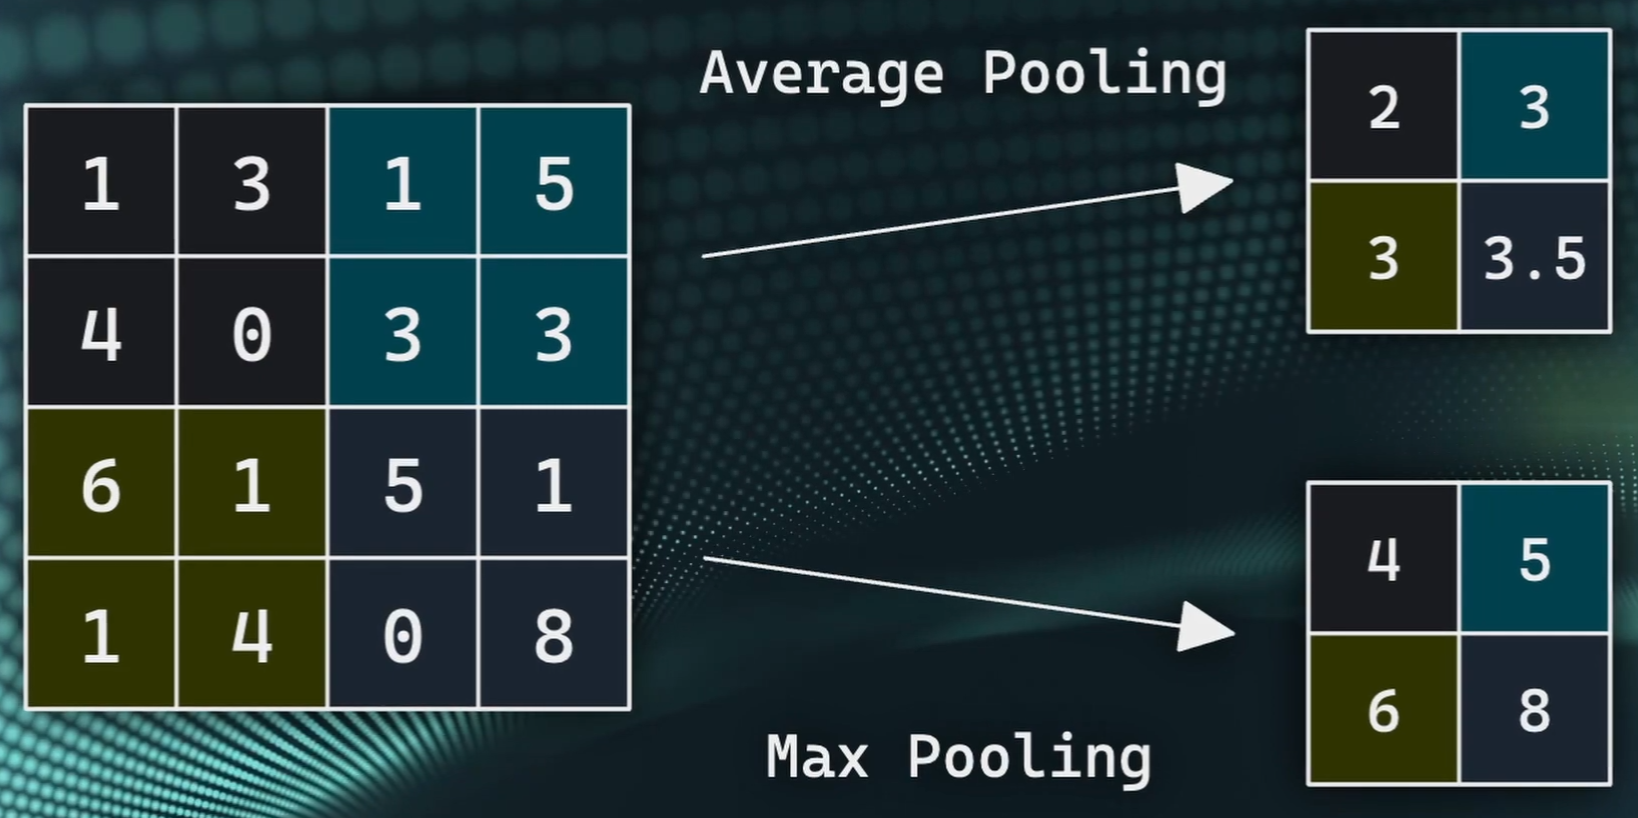
\includegraphics[width=0.95\textwidth,height=0.95\textheight,keepaspectratio]{images/cnn/pooling-layer.png}
    \end{figure}
\end{frame}

\begin{frame}[allowframebreaks]{Convolutions on RGB images}
    \begin{figure}
    \centering
    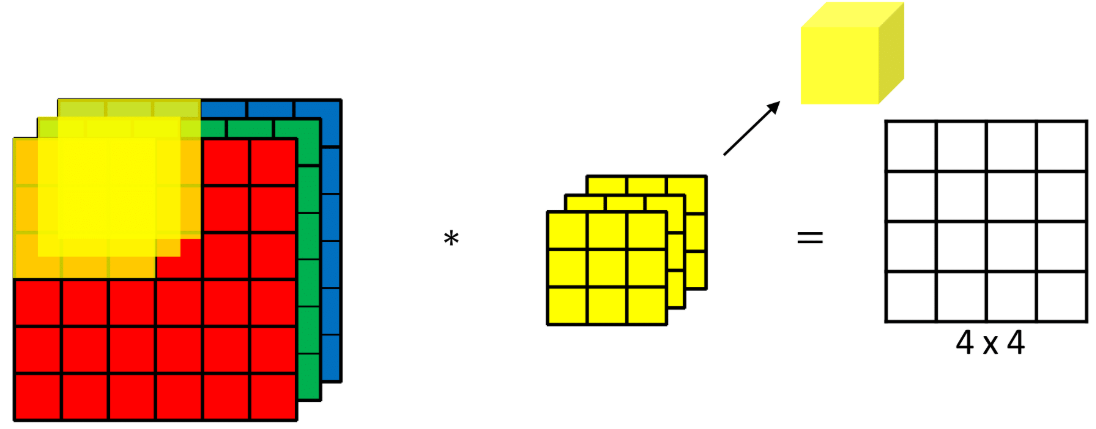
\includegraphics[width=0.95\textwidth,height=0.95\textheight,keepaspectratio]{images/cnn/rgb-convolution.png}
    \end{figure}
\end{frame}

\begin{frame}[allowframebreaks]{Multiple Channels \& Multiple Filters}
    \begin{figure}
    \centering
    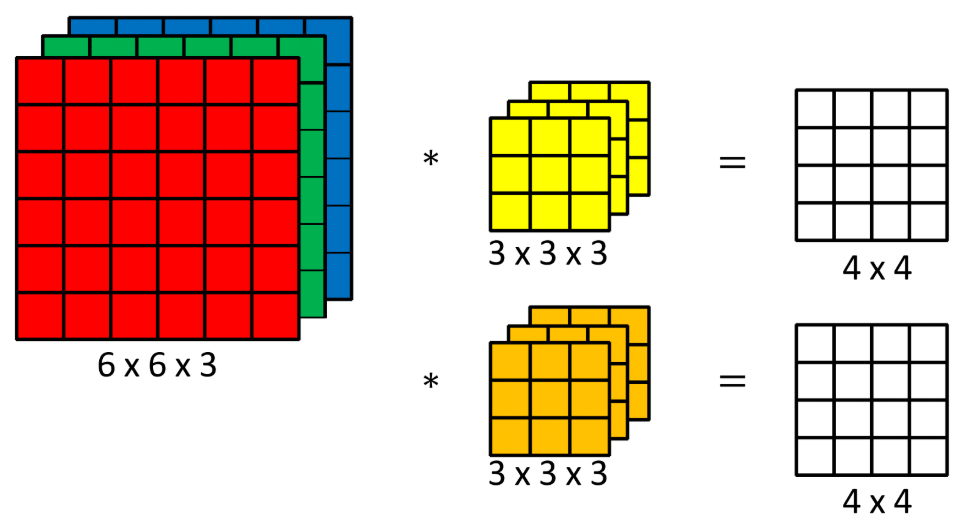
\includegraphics[width=0.95\textwidth,height=0.95\textheight,keepaspectratio]{images/cnn/mutiple-filters.png}
    \end{figure}
\end{frame}

\begin{frame}[allowframebreaks]{Number of Parameters?}
    \LARGE If you have 10 filters of size $3 \times 3 \times 3$ in one layer of a neural network, how many parameters does that layer have?

\framebreak
    Each filter has size $3 \times 3 \times 3 = 27$ parameters (weights).  \\[2em]
    With 10 filters: $10 \times 27 = 270$ weights.  \\[2em]
    If each filter also has a bias term, add 10 more parameters: \textbf{$270 + 10 = 280$} parameters in total.
\end{frame}
\begin{frame}[fragile]{CNN - Padding & Strides}
\begin{block}{Padding:}
    \begin{itemize}
        \item “same” preserves spatial size by adding zeros around input;
        \item “valid” reduces spatial size by not adding any padding.
        \item Padding is used to control the spatial size of the output feature map.
        \item Padding is added to the input image before applying the convolution operation.
    \end{itemize}
\end{block}

\begin{block}{Strides:}
    \begin{itemize}
        \item Strides control how much the filter moves across the input image.
        \item Strides can be set independently for height and width.
        \item Strides are used to control the spatial size of the output feature map.
        \item Strides are set in the convolutional layer.
    \end{itemize}
\end{block}

\begin{lstlisting}[language=Python, caption={Code snippet (PyTorch)}, basicstyle=\ttfamily\footnotesize]
import torch.nn as nn

conv_valid = nn.Conv2d(3, 16, 3, stride=2, padding=0) # “Valid”: no padding (padding=0)
conv_same  = nn.Conv2d(3, 16, 3, stride=1, padding=1) # “Same”: preserve size
\end{lstlisting}
\end{frame}  

% Add 4 images in a row with captions at the bottom
\begin{frame}{CNN - Padding & Strides}
    \begin{figure}
    \centering
    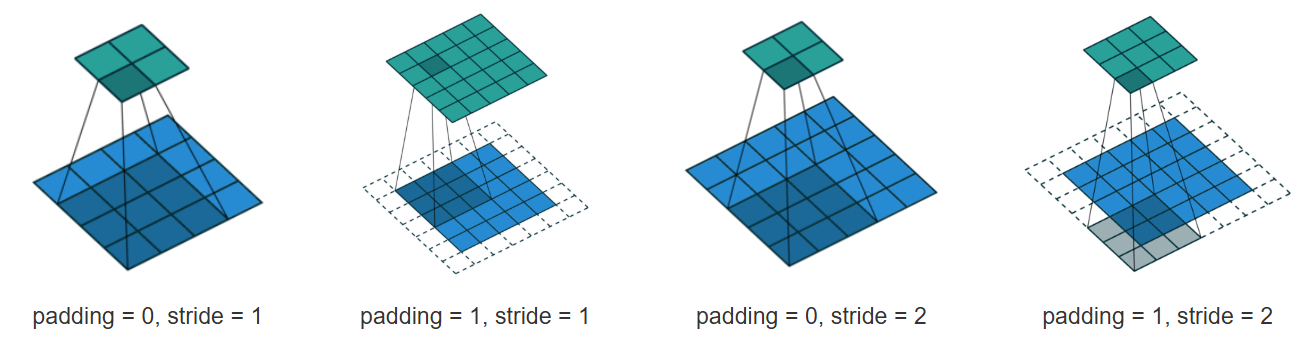
\includegraphics[width=1\textwidth,height=1\textheight,keepaspectratio]{images/cnn/padding-stride.png}
    \end{figure}
\end{frame}
\begin{frame}[fragile]{CNN - Normalization (Batch Norm)}
\begin{block}{What:}
    \begin{itemize}
        \item Normalize layer inputs over mini‑batch, then scale & shift.
    \end{itemize}
\end{block}

\begin{block}{Benefits:}
    \begin{itemize}
        \item Faster training,
        \item Allows higher learning rates,
        \item Reduces sensitivity to initialization,
        \item Acts as a regularizer.
    \end{itemize}
\end{block}

\begin{lstlisting}[language=Python, caption={Code snippet (PyTorch)}, basicstyle=\ttfamily\footnotesize]
import torch.nn as nn

bn = nn.BatchNorm2d(16)
x = bn(x)
\end{lstlisting}

\begin{block}{Note:}
    \begin{itemize}
        \item BatchNorm is typically used after convolutional layers and before activation functions.
        \item BatchNorm normalizes activations per‑batch, then scales/shifts them. 
    \end{itemize}
\end{block}
\end{frame}  

\begin{frame}{CNN - Normalization (Batch Norm)}
    \begin{figure}
    \centering
    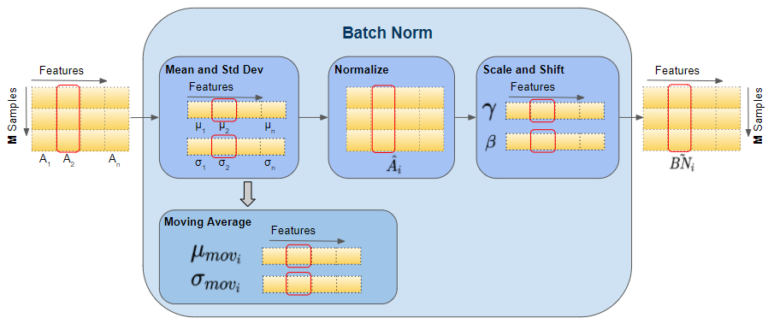
\includegraphics[width=0.95\textwidth,height=0.4\textheight,keepaspectratio]{images/cnn/batch-norm-unit.png}
    \end{figure}

    \begin{figure}
    \centering
    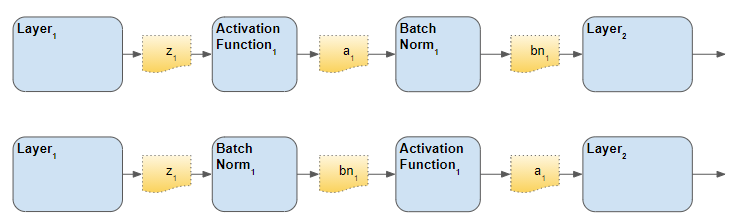
\includegraphics[width=0.95\textwidth,height=0.4\textheight,keepaspectratio]{images/cnn/batch-norm-sequence.png}
    \caption{Order of placement of Batch Norm layer}
    \end{figure}

    \href{https://towardsdatascience.com/batch-norm-explained-visually-how-it-works-and-why-neural-networks-need-it-b18919692739/}{More on Batch Norm from Towards Data Science}
\end{frame}
\begin{frame}{Regularization}

    \centering
    \Huge{\textbf{Regularization}}

    \vfill

    \small{Slides from: \url{https://harvard-iacs.github.io/2019-CS109A/lectures/lecture8/presentation/Lecture8a_Regularization.pptx}}

\end{frame}

\begin{frame}{Regularization: An Overview}
    \begin{itemize}
        \item Regularization involves modifying the loss function $L$ to improve model generalization.
        \item A regularization term is added to penalize certain properties of the model parameters:
        \[
            L_{\text{reg}}(\beta) = L(\beta) + \lambda R(\beta)
        \]
        \item $\lambda$ is a scalar that controls the strength of the regularization.
        \item The function $R(\beta)$ encodes the properties to penalize (e.g., large coefficients).
        \item Minimizing $L_{\text{reg}}$ leads to model parameters with more desirable characteristics.
    \end{itemize}
\end{frame}


\begin{frame}[allowframebreaks]{LASSO Regression}
    \begin{itemize}
        \item LASSO discourages extreme values in model parameters by penalizing their magnitudes.
        \item We use MSE as the base loss function.
        \item The regularized loss function is:
        \[
            L_{\text{LASSO}}(\beta) = \frac{1}{n} \sum_{i=1}^{n} \left| y_i - \beta^\top x_i \right|^2 + \lambda \sum_{j=1}^{J} |\beta_j|
        \]
        \item The term \( \sum_{j=1}^{J} |\beta_j| \) is the \( \ell_1 \) norm of the vector \( \beta \):
        \[
            \sum_{j=1}^{J} |\beta_j| = \|\beta\|_1
        \]
    \end{itemize}
\end{frame}

\begin{frame}[allowframebreaks]{Ridge Regression}
    \begin{itemize}
        \item Regularization term penalizes the \textbf{squares} of the parameter magnitudes.
        \item The regularized loss function becomes:
        \[
            L_{\text{Ridge}}(\beta) = \frac{1}{n} \sum_{i=1}^{n} \left| y_i - \beta^\top x_i \right|^2 + \lambda \sum_{j=1}^{J} \beta_j^2
        \]
        \item Note that:
        \[
            \sum_{j=1}^{J} \beta_j^2 = \|\beta\|_2^2
        \]
        which is the square of the \( \ell_2 \)-norm of \( \beta \).
    \end{itemize}
\end{frame}


\begin{frame}{Choosing \( \lambda \)}
    \begin{itemize}
        \item In both ridge and LASSO regression, the larger the regularization parameter \( \lambda \), the more we penalize large values in \( \beta \).
        \item If \( \lambda \) is close to zero:
        \begin{itemize}
            \item The penalty is minimal.
            \item We recover the MSE, i.e., ridge and LASSO become ordinary regression.
        \end{itemize}
        \item If \( \lambda \) is sufficiently large:
        \begin{itemize}
            \item The MSE term becomes negligible.
            \item The regularization forces \( \beta_{\text{ridge}} \) and \( \beta_{\text{LASSO}} \) close to zero.
        \end{itemize}
        \item To avoid ad-hoc selection, \( \lambda \) should be chosen via cross-validation.
    \end{itemize}
\end{frame}


\begin{frame}{Ridge, LASSO - Computational Complexity}
    \begin{itemize}
        \item \textbf{Ridge Regression Solution:}
        \[
            \beta = (X^T X + \lambda I)^{-1} X^T Y
        \]
        
        \item \textbf{LASSO Regression:}
        \begin{itemize}
            \item No closed-form analytical solution.
            \item The \( L_1 \) norm is not differentiable at 0.
            \item We use the concept of \textit{subdifferential} or \textit{subgradient} to derive manageable expressions.

        \end{itemize}
    \end{itemize}
\end{frame}


\begin{frame}{Regularization Parameter with a Validation Set}
    The solution of the Ridge/Lasso regression involves three steps:
    \begin{itemize}
        \item Select \( \lambda \)
        \item Find the minimum of the ridge/Lasso regression loss function (using the ridge formula), and record the \textbf{MSE on the validation/test set}.
        \item Find the \( \lambda \) that gives the smallest \( \text{MSE} \)
    \end{itemize}
\end{frame}


\begin{frame}{The Geometry of Regularization (LASSO)}
    \begin{itemize}
        \item[] \[
        L_{\text{LASSO}}(\boldsymbol{\beta}) = \frac{1}{n} \sum_{i=1}^n \left| y_i - \boldsymbol{\beta}^T \mathbf{x} \right|^2 + \lambda \sum_{j=1}^J |\beta_j|
        \]
        \item[] \[
        \hat{\boldsymbol{\beta}}^{\text{LASSO}} = \arg\min L_{\text{LASSO}}(\boldsymbol{\beta})
        \]
    \end{itemize}

    \begin{figure}
        \centering
        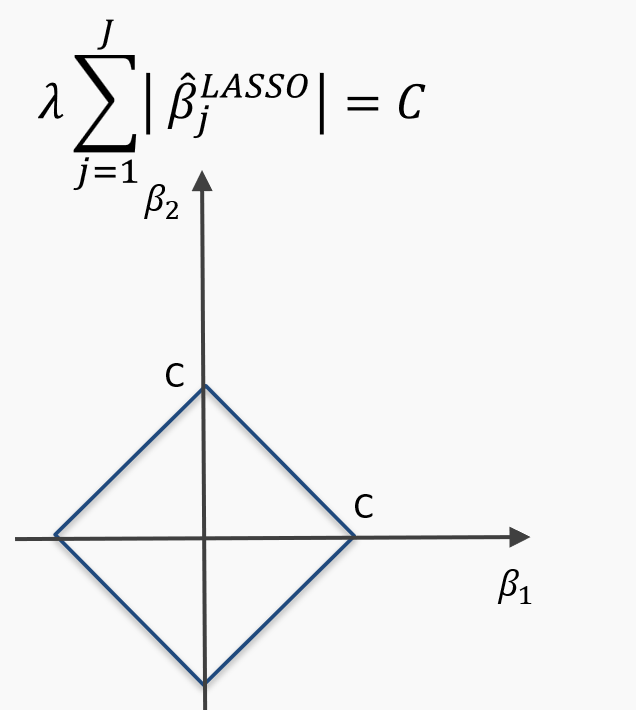
\includegraphics[width=0.35\textwidth]{images/linear-regression/linear-regression-22.png}
        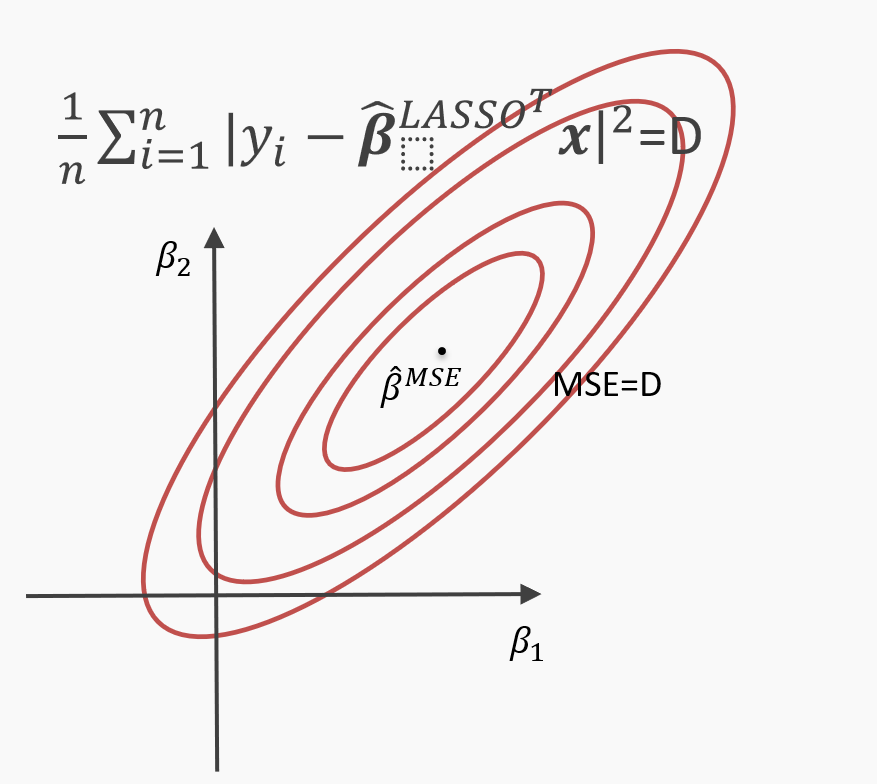
\includegraphics[width=0.35\textwidth]{images/linear-regression/linear-regression-23.png}
    \end{figure}
\end{frame}


\begin{frame}{The Geometry of Regularization (LASSO)}
    \begin{itemize}
        \item Regularized loss function:
        \[
            L_{\text{LASSO}}(\boldsymbol{\beta}) = \frac{1}{n} \sum_{i=1}^{n} \left| y_i - \boldsymbol{\beta}^T \mathbf{x} \right|^2 + \lambda \sum_{j=1}^{J} |\beta_j|
        \]
        \item LASSO solution:
        \[
            \hat{\boldsymbol{\beta}}^{\text{LASSO}} = \arg\min L_{\text{LASSO}}(\boldsymbol{\beta})
        \]
    \end{itemize}

    \vspace{1em}

    \begin{columns}
        \column{0.5\textwidth}
        \begin{itemize}
            \item $L_1 = \lambda \sum_{j=1}^{J} \left| \hat{\beta}_j^{\text{LASSO}} \right|$
        \end{itemize}
        \begin{center}
            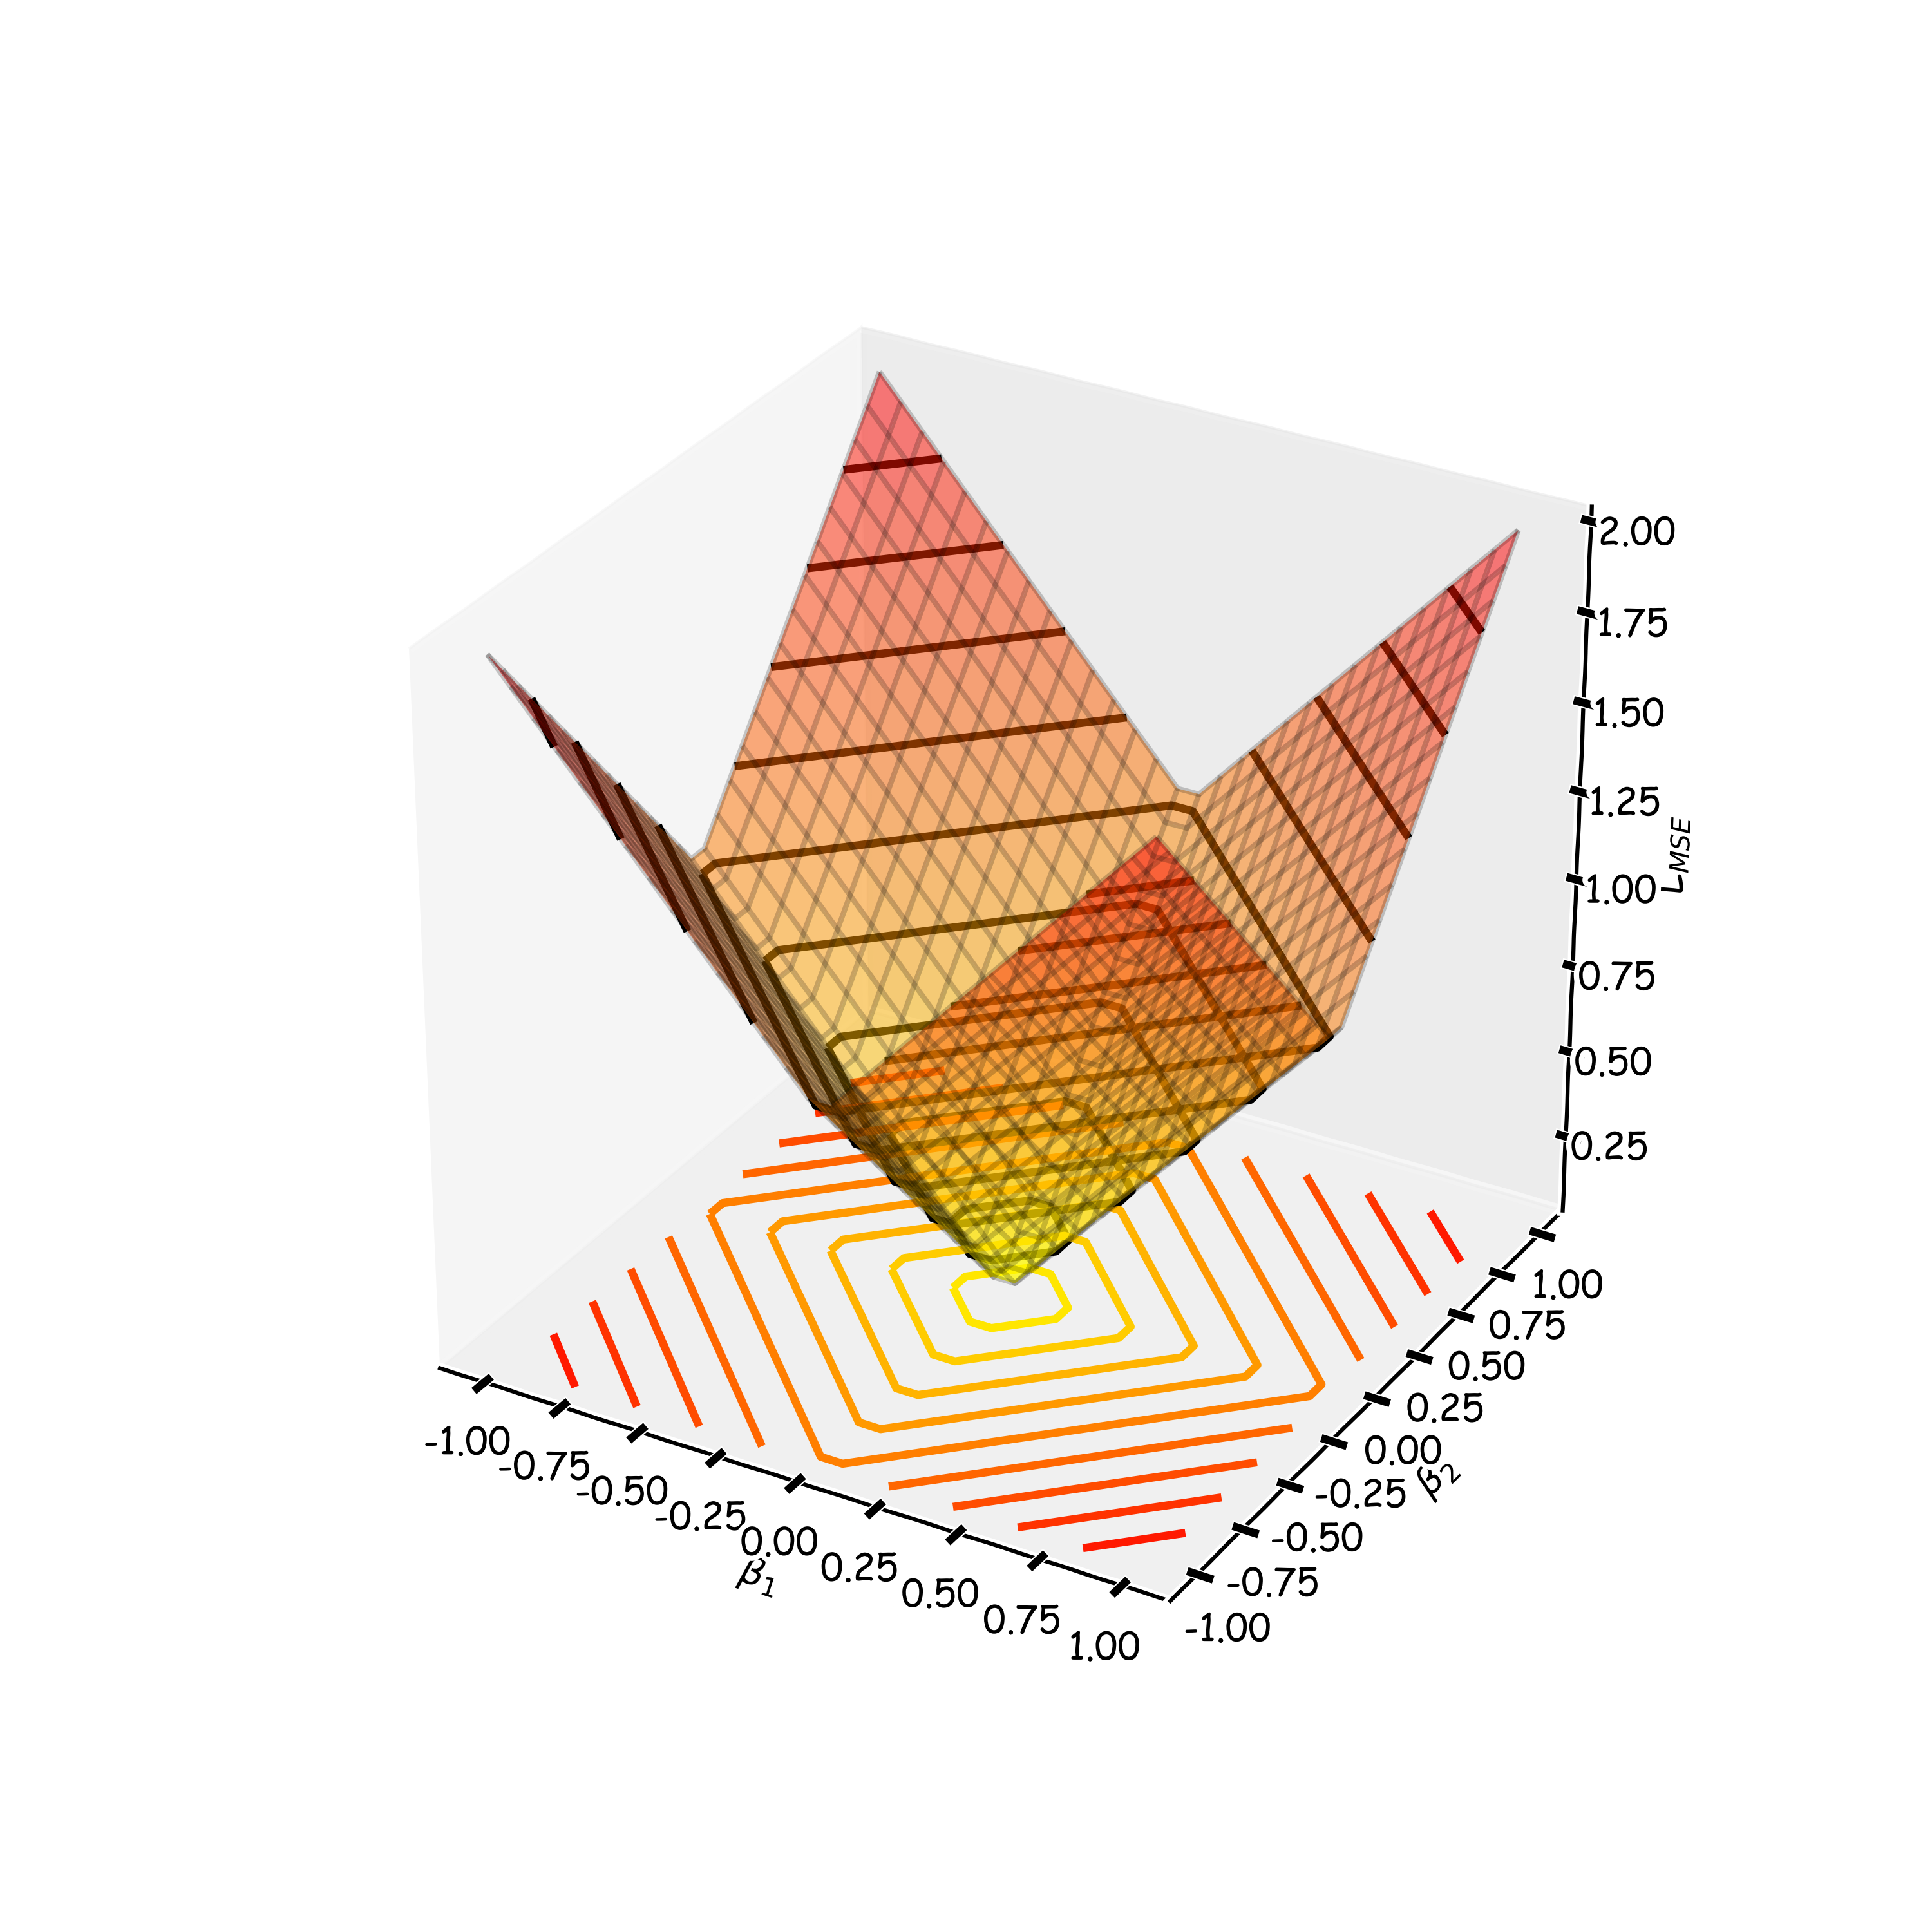
\includegraphics[height=3.5cm]{images/linear-regression/linear-regression-24.png}
        \end{center}

        \column{0.5\textwidth}
        \begin{itemize}
            \item $L_{\text{MSE}}(\boldsymbol{\beta}) = \frac{1}{n} \sum_{i=1}^{n} \left| y_i - \boldsymbol{\beta}^T \mathbf{x} \right|^2$
        \end{itemize}
        \begin{center}
            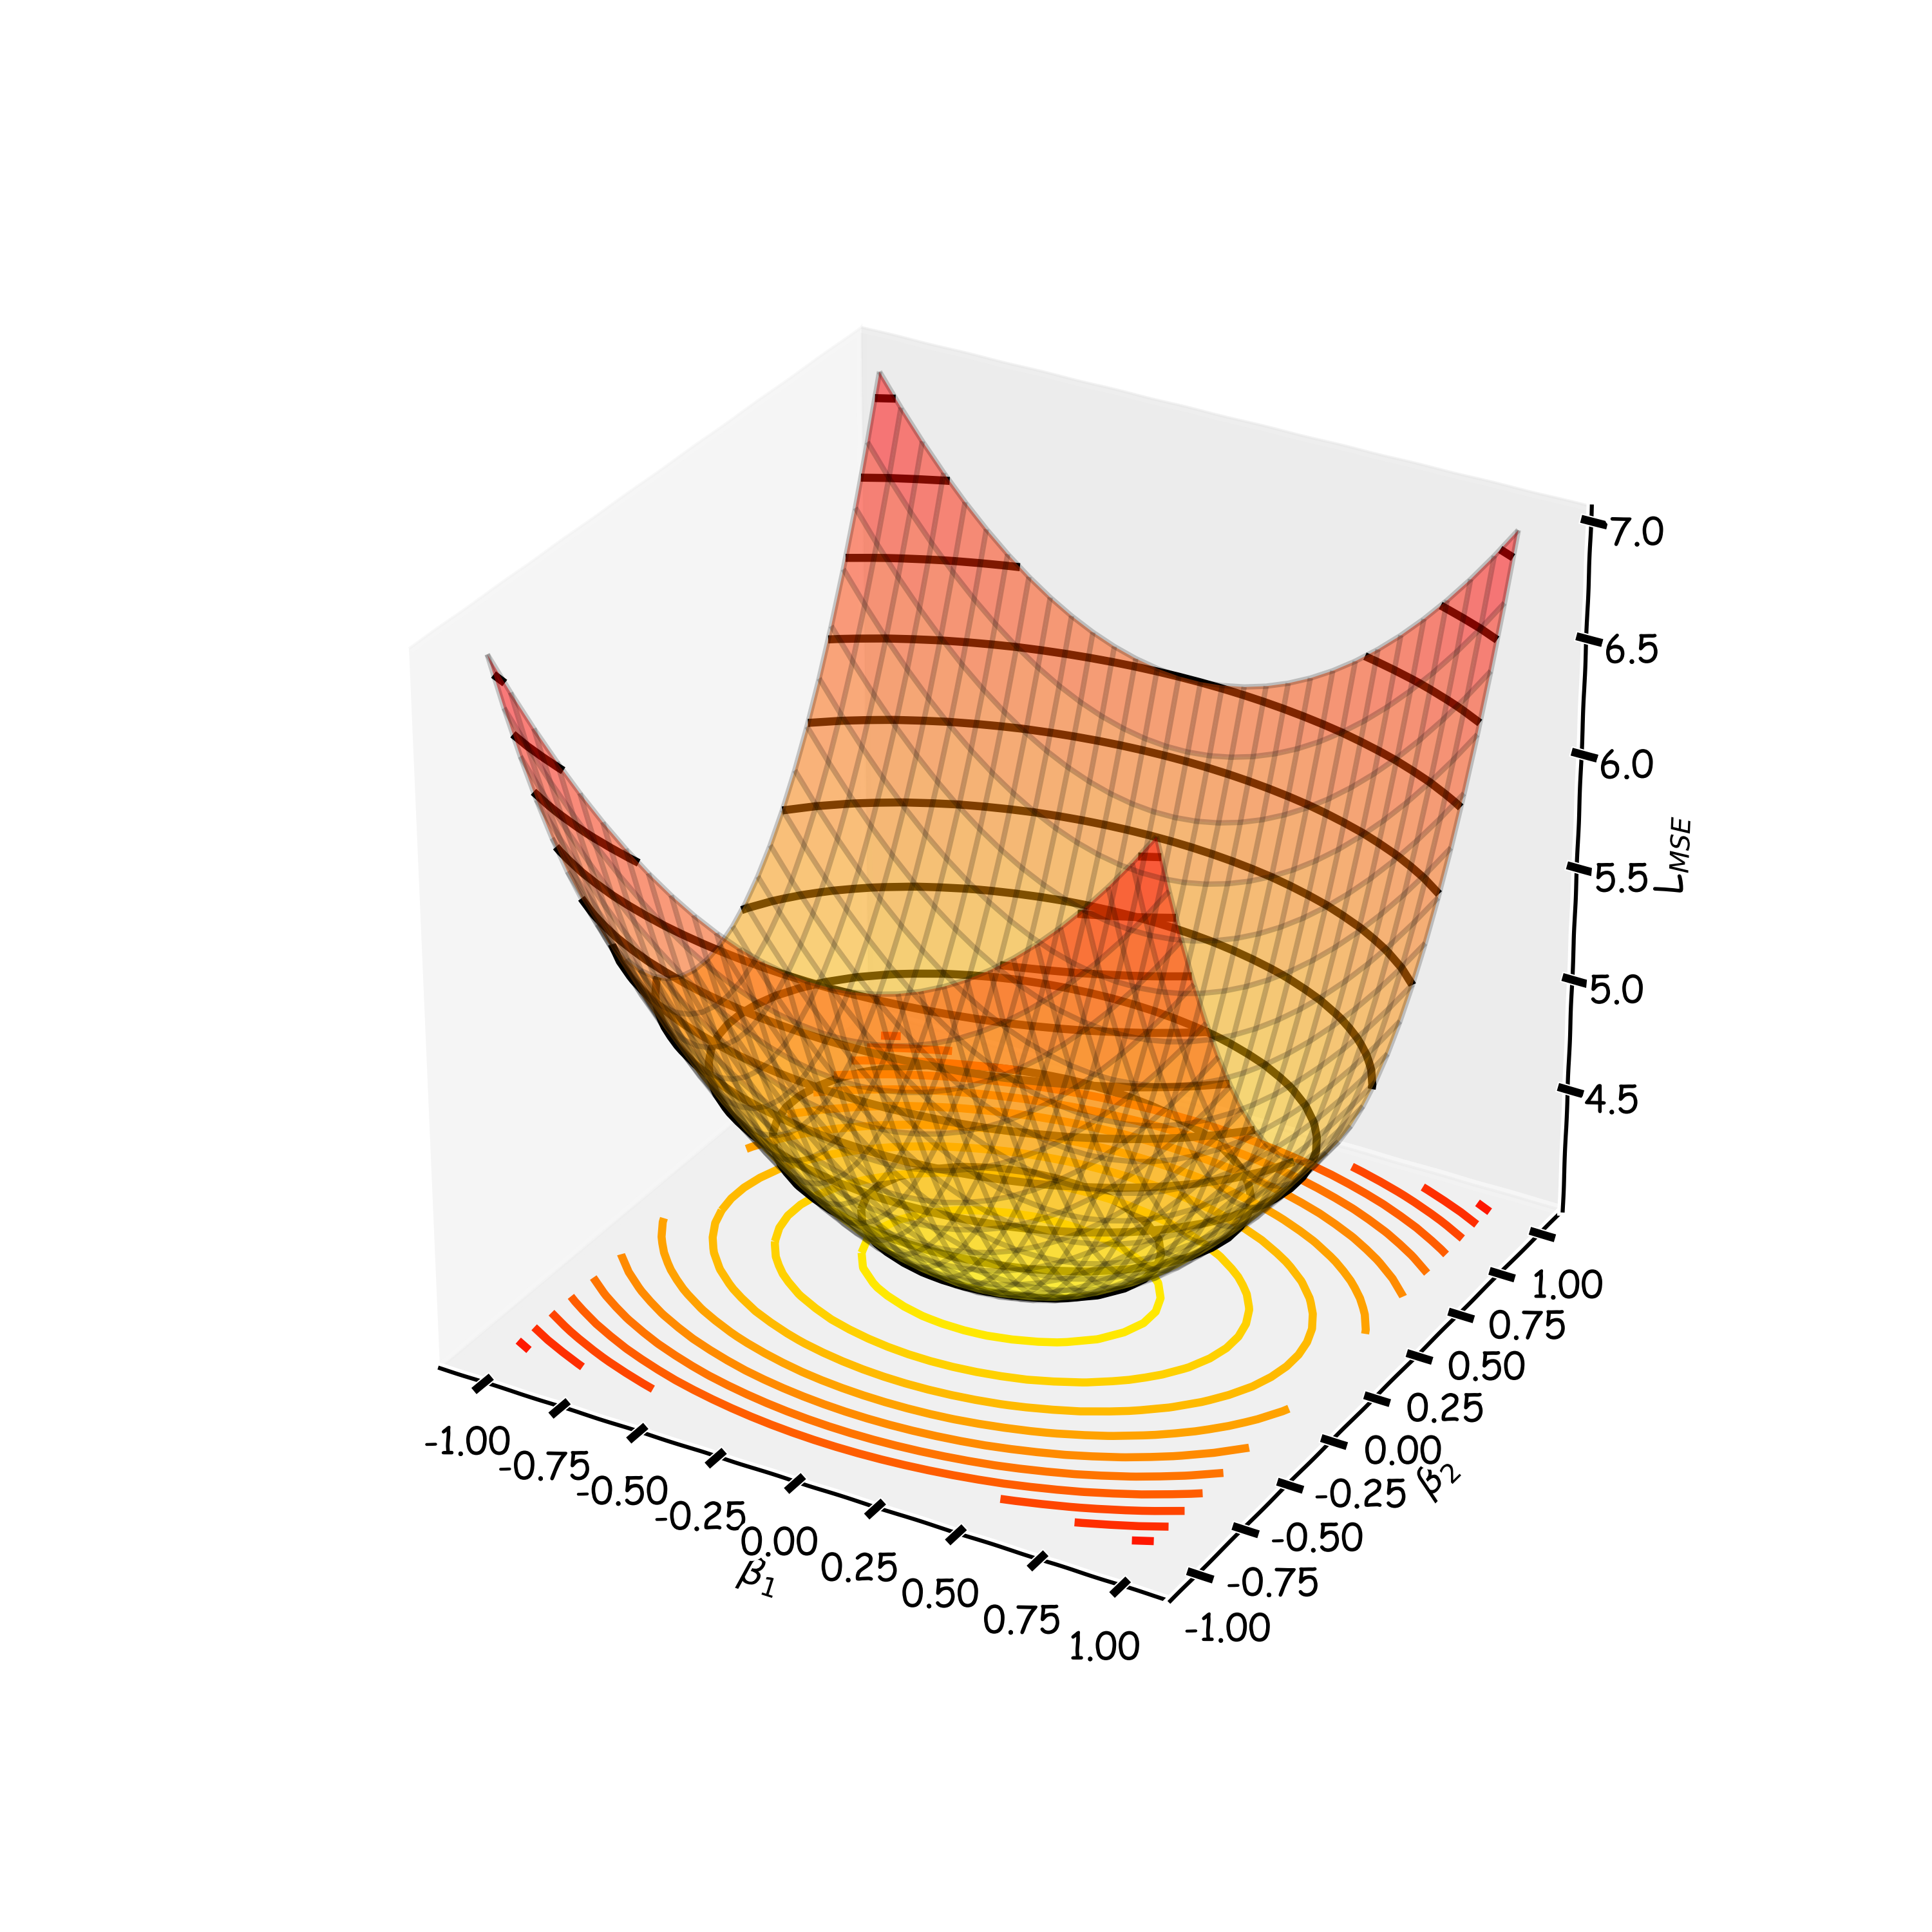
\includegraphics[height=3.5cm]{images/linear-regression/linear-regression-25.png}
        \end{center}
    \end{columns}
\end{frame}


\begin{frame}{LASSO visualized}
    \begin{columns}
        \column{0.5\textwidth}
        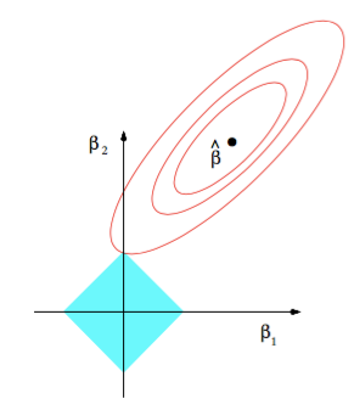
\includegraphics[height=4cm]{images/linear-regression/linear-regression-26.png}
        \begin{itemize}
            \item The LASSO estimator tends to zero out parameters.
            \item The OLS loss can easily intersect with the constraint on one of the axes.
        \end{itemize}

        \column{0.5\textwidth}
        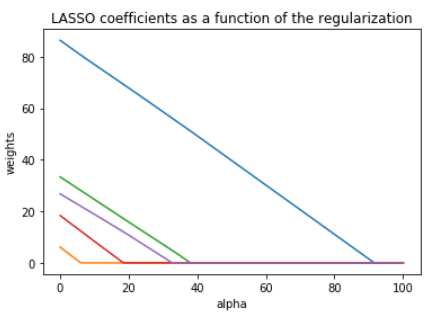
\includegraphics[height=4cm]{images/linear-regression/linear-regression-27.png}
        \begin{itemize}
            \item The values of the coefficients decrease as $\lambda$ increases.
            \item Coefficients are nullified quickly.
        \end{itemize}
    \end{columns}
\end{frame}


\begin{frame}{The Geometry of Regularization (Ridge)}

\begin{columns}
    \column{0.48\textwidth}
    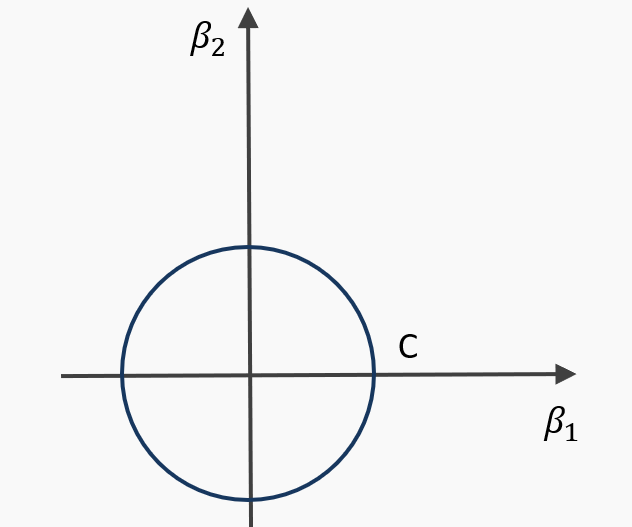
\includegraphics[width=\linewidth]{images/linear-regression/linear-regression-28.png}

    \begin{itemize}
        \item $L_{Ridge}(\boldsymbol{\beta}) = \frac{1}{n} \sum_{i=1}^n \left| y_i - \boldsymbol{\beta}^T \boldsymbol{x} \right|^2 + \lambda \sum_{j=1}^J (\beta_j)^2$
        \item $\hat{\boldsymbol{\beta}}^{Ridge} = \arg\min L_{Ridge}(\boldsymbol{\beta})$
        \item $\lambda \sum_{j=1}^J \left| \hat{\beta}_j^{Ridge} \right|^2 = C$
    \end{itemize}

    \column{0.48\textwidth}
    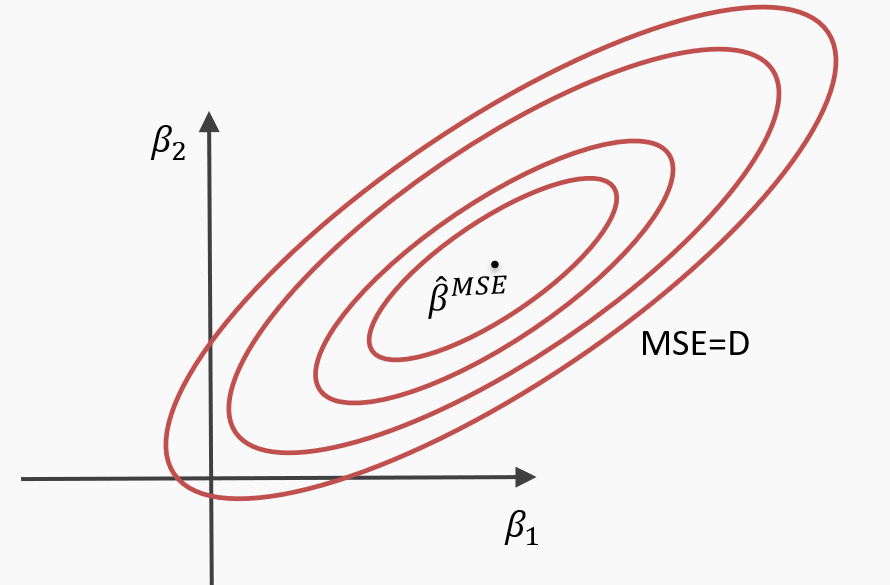
\includegraphics[width=\linewidth]{images/linear-regression/linear-regression-29.png}

    \begin{itemize}
        \item $\frac{1}{n} \sum_{i=1}^n \left| y_i - \hat{\boldsymbol{\beta}}^{Ridge\, T} \boldsymbol{x} \right|^2 = D$
        \item The ridge constraint forms a circle in 2D.
        \item The solution lies at the point where the MSE contour touches the constraint boundary.
    \end{itemize}

\end{columns}

\end{frame}


\begin{frame}{Ridge visualized}

\begin{columns}
    \column{0.48\textwidth}
    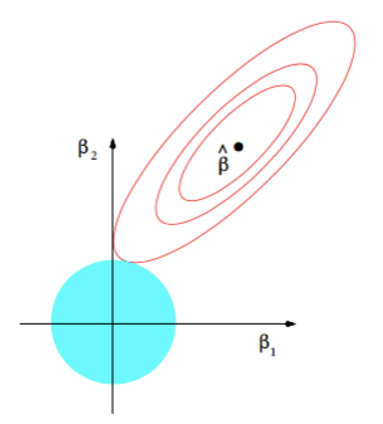
\includegraphics[width=\linewidth]{images/linear-regression/linear-regression-30.png}
    \begin{itemize}
        \item The ridge estimator is where the constraint and the loss intersect.
    \end{itemize}

    \column{0.48\textwidth}
    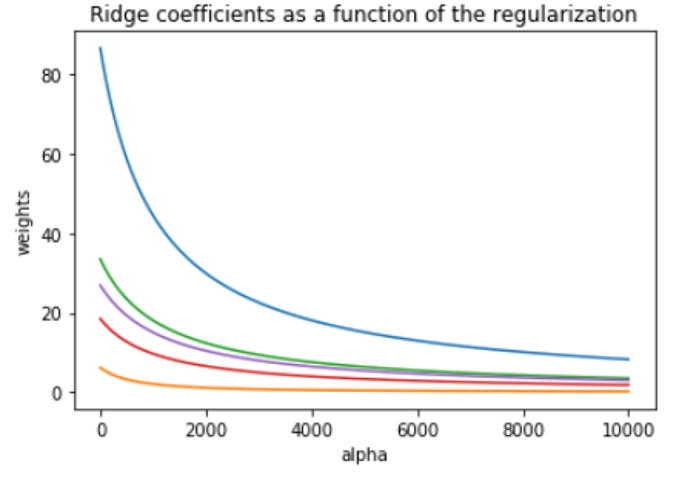
\includegraphics[width=\linewidth]{images/linear-regression/linear-regression-31.png}
    \begin{itemize}
        \item The values of the coefficients decrease as lambda increases, but they are not nullified.
    \end{itemize}
\end{columns}

\end{frame}


\begin{frame}{The Geometry of Regularization}

\begin{center}
    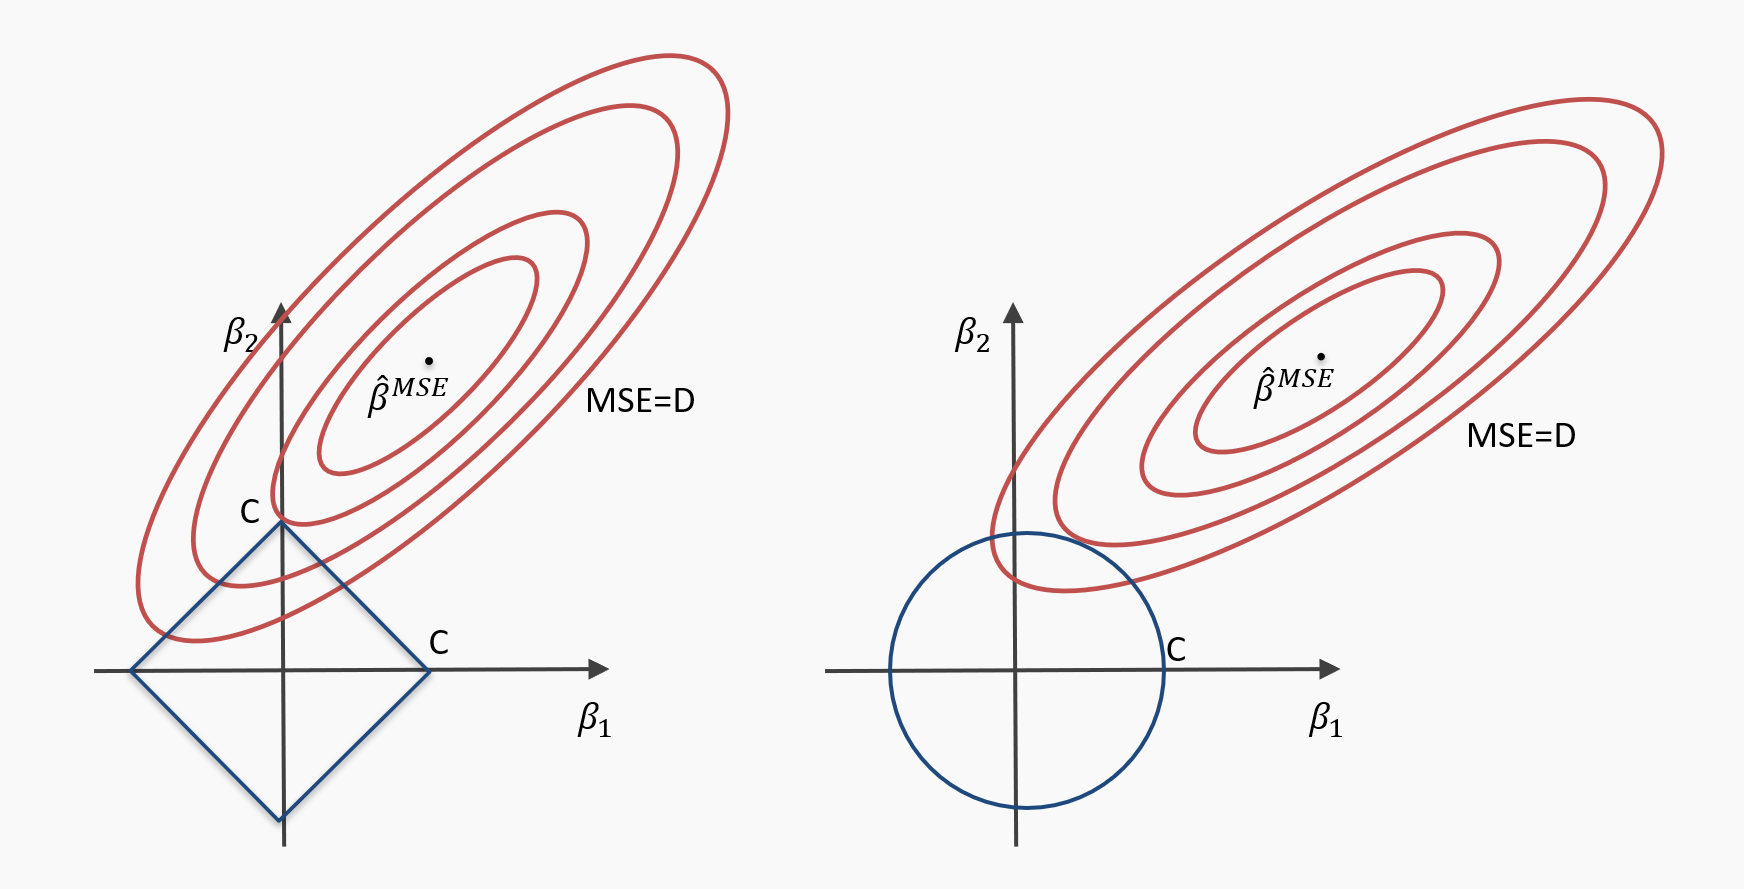
\includegraphics[width=0.9\linewidth]{images/linear-regression/linear-regression-32.png}
\end{center}

\end{frame}


\begin{frame}{Ridge regularization with only \textbf{validation}: step by step}
\begin{enumerate}
  \item Split data into $\{\{X, Y\}_{\text{train}}, \{X, Y\}_{\text{validation}}, \{X, Y\}_{\text{test}}\}$
  
  \item For $\lambda$ in $\{\lambda_{\min}, \dots, \lambda_{\max}\}$:
  \begin{enumerate}
    \item Determine the $\beta$ that minimizes the $L_{\text{ridge}}$:
    \[
    \hat{\beta}_{\text{Ridge}}(\lambda) = (X^T X + \lambda I)^{-1} X^T Y, \quad \text{using the train data}
    \]
    \item Record $L_{\text{MSE}}(\lambda)$ using validation data.
  \end{enumerate}
  
  \item Select the $\lambda$ that minimizes the loss on the validation data:
  \[
  \lambda_{\text{ridge}} = \arg\min_{\lambda} L_{\text{MSE}}(\lambda)
  \]
  
  \item Refit the model using both \textbf{train and validation} data:
  \[
  \{X, Y\}_{\text{train}}, \{X, Y\}_{\text{validation}} \Rightarrow \hat{\beta}_{\text{ridge}}(\lambda_{\text{ridge}})
  \]
  
  \item Report MSE or $R^2$ on $\{X, Y\}_{\text{test}}$ given the $\hat{\beta}_{\text{ridge}}(\lambda_{\text{ridge}})$
\end{enumerate}
\end{frame}


\begin{frame}{Lasso regularization with \textbf{validation only}: step by step}
\begin{enumerate}
    \item Split data into $\{ \{X, Y\}_{\text{train}}, \{X, Y\}_{\text{validation}}, \{X, Y\}_{\text{test}} \}$
    \item For $\lambda$ in $\{\lambda_{\min}, \dots, \lambda_{\max}\}$:
    \begin{enumerate}
        \item Determine the $\beta$ that minimizes the $L_{\text{lasso}}$,
        \[
        \hat{\beta}_{\text{lasso}}(\lambda),
        \]
        using the train data. \textbf{This is done using a solver}.
        \item Record $L_{\text{MSE}}(\lambda)$ using validation data.
    \end{enumerate}
    \item Select the $\lambda$ that minimizes the loss on the validation data:
    \[
    \lambda_{\text{lasso}} = \arg\min_{\lambda} L_{\text{MSE}}(\lambda)
    \]
    \item Refit the model using both \textbf{train} and \textbf{validation} data:
    \[
    \{X, Y\}_{\text{train}}, \{X, Y\}_{\text{validation}} \Rightarrow \hat{\beta}_{\text{lasso}}(\lambda_{\text{lasso}})
    \]
    \item Report MSE or $R^2$ on $\{X, Y\}_{\text{test}}$ given the $\hat{\beta}_{\text{lasso}}(\lambda_{\text{lasso}})$
\end{enumerate}
\end{frame}


\begin{frame}{Ridge regularization with \textbf{validation only}: step by step}
\centering
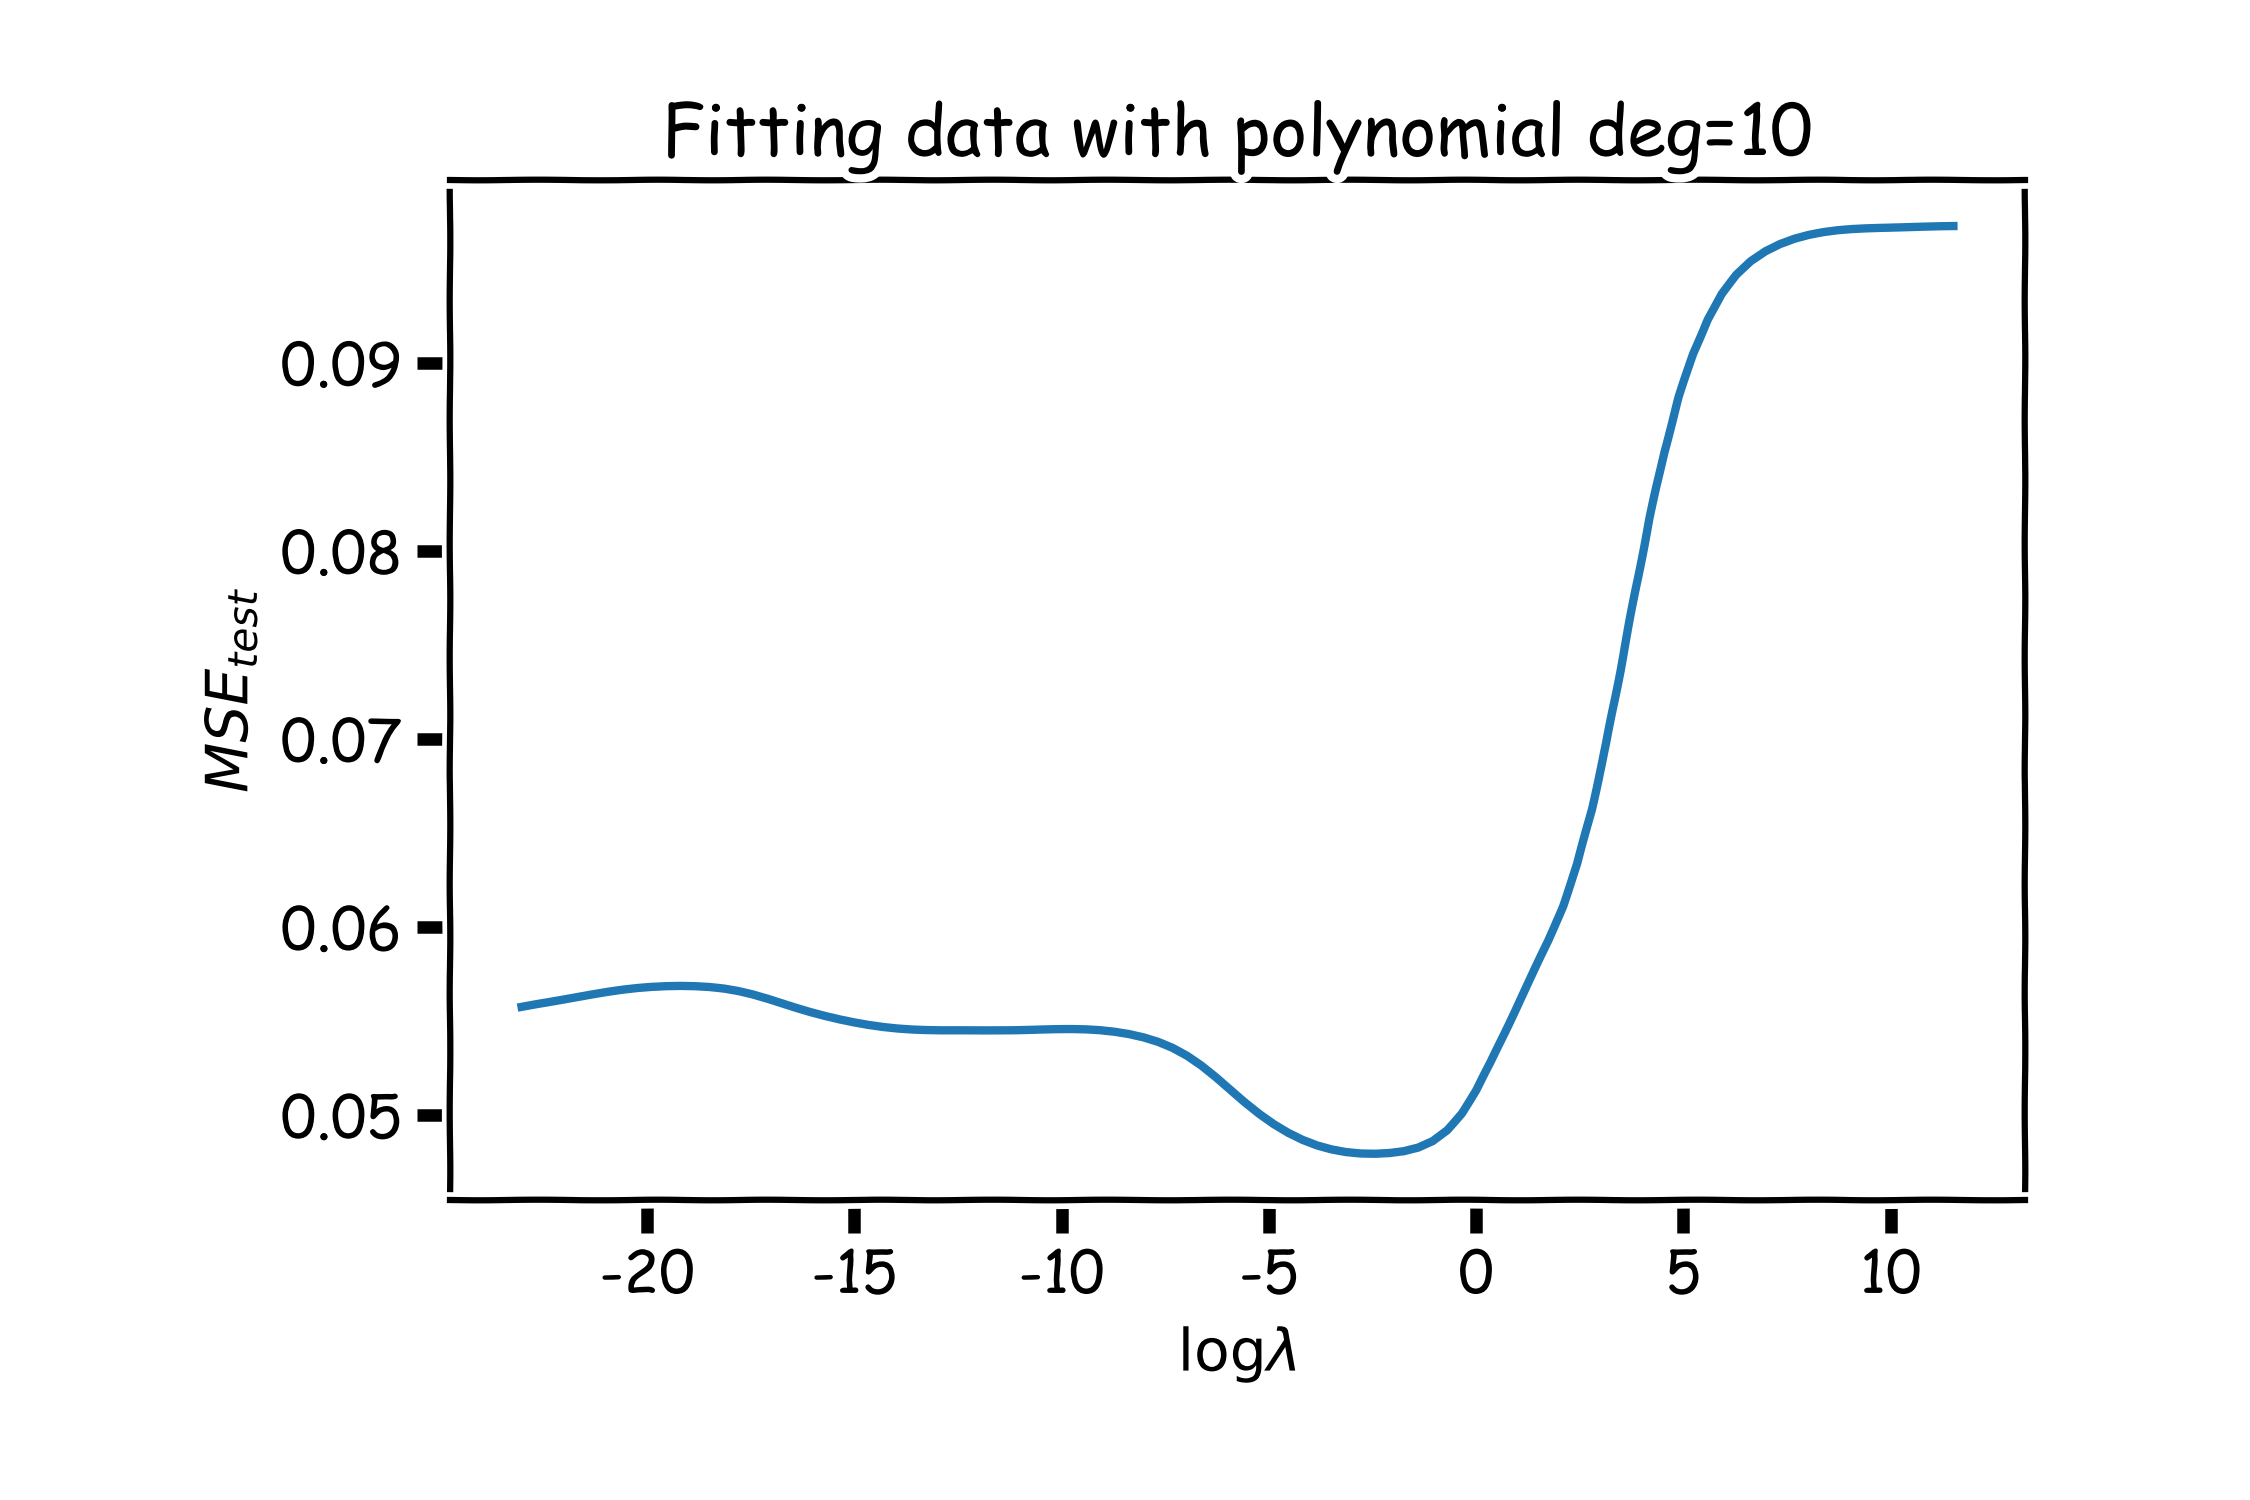
\includegraphics[width=0.85\linewidth]{images/linear-regression/linear-regression-33.png}

\end{frame}


\begin{frame}[allowframebreaks]{Ridge regularization with \textbf{CV}: step by step}
\begin{enumerate}
    \item Remove $\{X, Y\}_{\text{test}}$ from data.
    \item Split the rest of the data into $K$ folds:  
    $\left\{\{X, Y\}_{\text{train}}^{-k}, \{X, Y\}_{\text{val}}^k\right\}$
    
    \item For $k \in \{1, \dots, K\}$:
    \begin{enumerate}
        \item For $\lambda \in \{\lambda_0, \dots, \lambda_n\}$:
        \begin{itemize}
            \item Determine the $\beta$ that minimizes the $L_{\text{ridge}}$:
            \[
            \hat{\beta}_{\text{ridge}}(\lambda, k) = (X^\top X + \lambda I)^{-1} X^\top Y
            \]
            using the training data $\{X, Y\}_{\text{train}}^k$.
            \item Record $L_{\text{MSE}}(\lambda, k)$ using the validation data $\{X, Y\}_{\text{val}}^k$.
        \end{itemize}
    \end{enumerate}
    At this point, we have a 2D matrix: rows correspond to different $k$, and columns to different $\lambda$ values.

    \item Average the $L_{\text{MSE}}(\lambda, k)$ for each $\lambda$:
    \[
    \bar{L}_{\text{MSE}}(\lambda) = \frac{1}{K} \sum_{k=1}^{K} L_{\text{MSE}}(\lambda, k)
    \]

    \item Find the $\lambda$ that minimizes $\bar{L}_{\text{MSE}}(\lambda)$:  
    $\lambda_{\text{ridge}} = \arg\min_\lambda \bar{L}_{\text{MSE}}(\lambda)$

    \item Refit the model using the full training data  
    $\left\{\{X, Y\}_{\text{train}}, \{X, Y\}_{\text{val}}\right\} \Rightarrow \hat{\beta}_{\text{ridge}}(\lambda_{\text{ridge}})$

    \item Report MSE or $R^2$ on $\{X, Y\}_{\text{test}}$ using $\hat{\beta}_{\text{ridge}}(\lambda_{\text{ridge}})$
\end{enumerate}
\end{frame}


\begin{frame}{Ridge regularization with \textbf{CV} only: step by step}
\begin{figure}
    \centering
    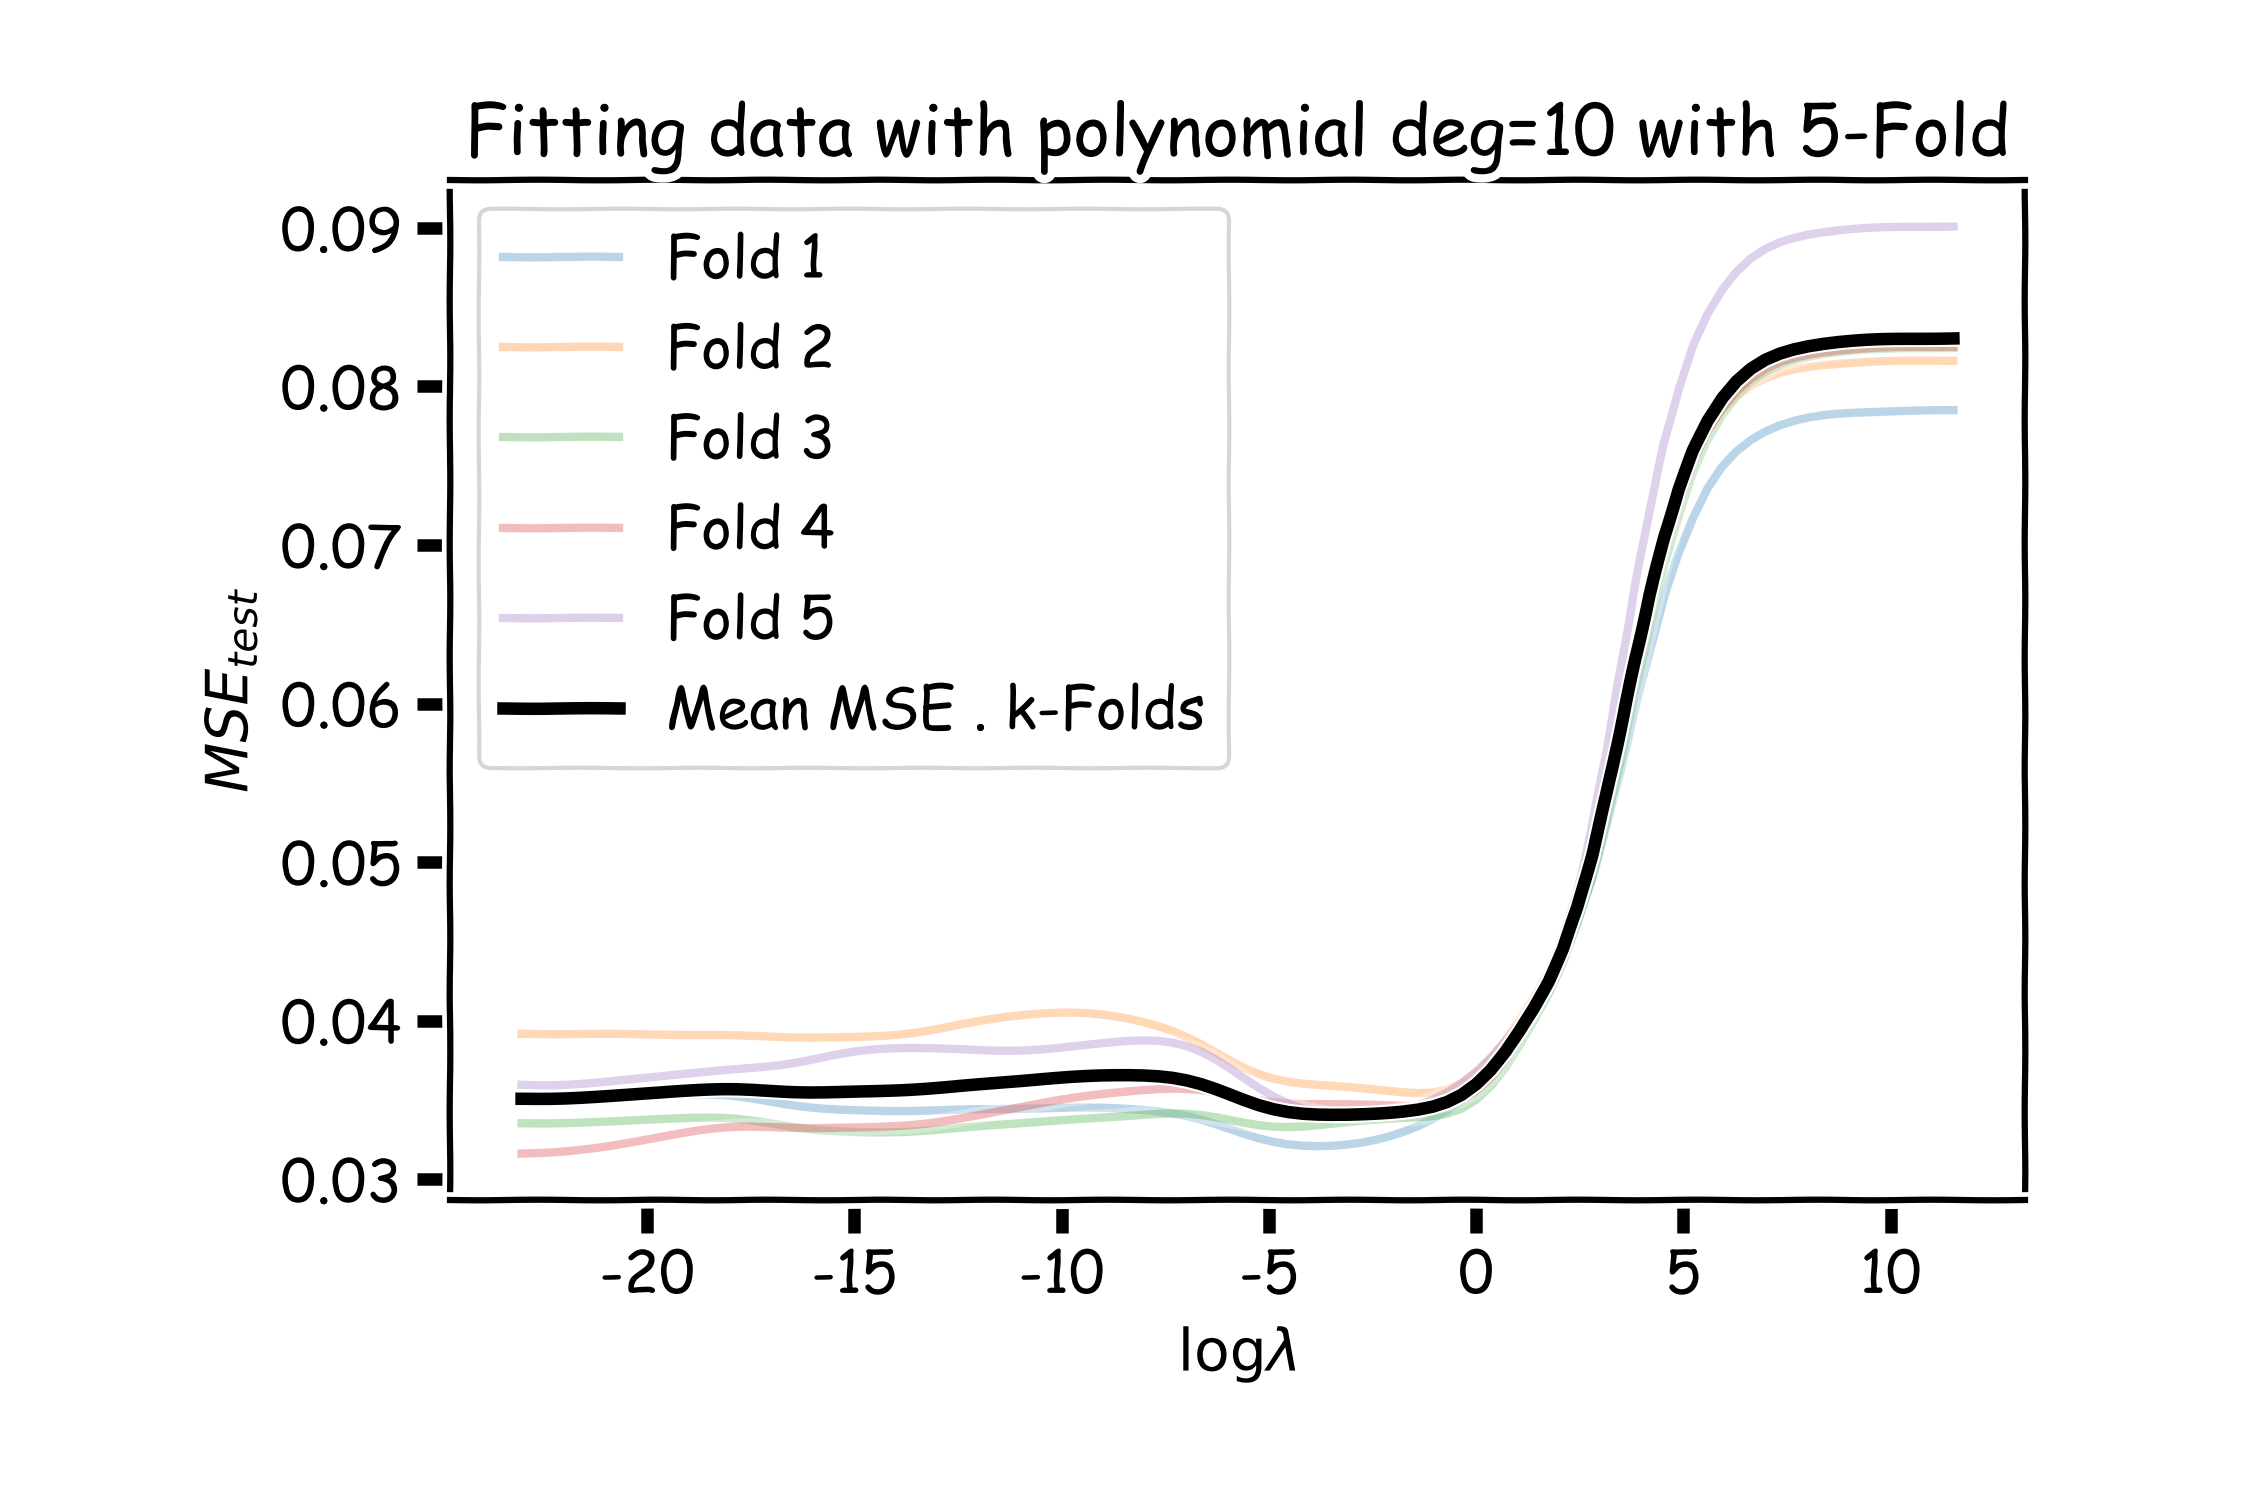
\includegraphics[width=0.9\textwidth]{images/linear-regression/linear-regression-34.png}
    \caption*{
        \small
        Validation error $MSE_{\text{val}}$ across $\lambda$ values (log scale) using 5-fold cross-validation. \\
        Each colored line corresponds to one fold. The thick black curve shows the mean validation error across all folds.
    }
\end{figure}
\end{frame}


\begin{frame}{Variable Selection as Regularization}

\begin{itemize}
    \item Since \textbf{LASSO} regression tends to produce zero estimates for a number of model parameters – we say that LASSO solutions are \textbf{sparse} – we consider LASSO to be a method for variable selection.
    
    \item Many prefer using LASSO for variable selection (as well as for suppressing extreme parameter values) rather than stepwise selection, as LASSO avoids the statistical problems that arise in stepwise selection.
    
    \item \textbf{Question:} What are the pros and cons of the two approaches?
\end{itemize}

\end{frame}

\begin{frame}[fragile]{CNN - Flattening & Fully Connected Layers}
\begin{block}{Flatten:}
    \begin{itemize}
        \item Flattening is the process of converting a multi-dimensional tensor into a one-dimensional tensor.
        \item Flattening is typically done before passing the data to fully connected layers.
    \end{itemize}
\end{block}

\begin{block}{FC Layer:}
    \begin{itemize}
        \item Used to learn complex relationships between features.
        \item Typically used at the end of the network to make predictions.
        \item Take the flattened output from the previous layer and produce a vector of class scores.
        \item Are often followed by activation functions like ReLU or softmax.
    \end{itemize}
\end{block}

\begin{lstlisting}[language=Python, caption={Code snippet (PyTorch)}, basicstyle=\ttfamily\footnotesize]
import torch.nn as nn
import torch

x = torch.flatten(x, 1)  # preserve batch dim
fc = nn.Linear(in_features=16*8*8, out_features=10)
out = fc(x)
\end{lstlisting}
\end{frame}  

\begin{frame}{CNN - Flattening & Fully Connected Layers}
\begin{figure}
\centering
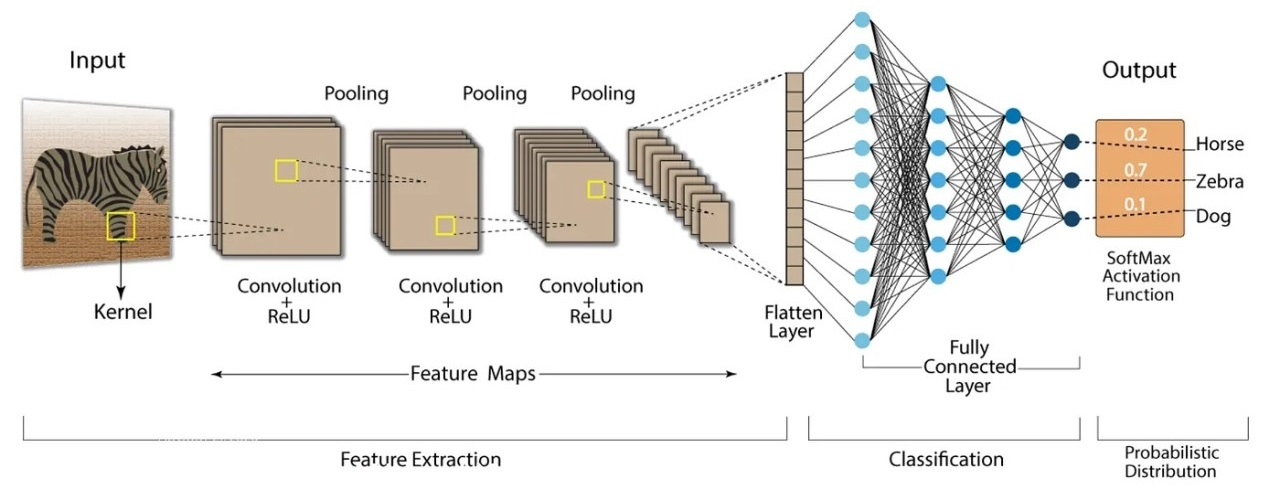
\includegraphics[width=1.0\textwidth,height=0.9\textheight,keepaspectratio]{images/cnn/cnn-fully-connected.jpeg}
\end{figure}
    
\end{frame}
\begin{frame}[fragile, allowframebreaks]{CNN - Loss Functions & Optimizers}
\begin{block}{Loss:}
    \begin{itemize}
        \item Loss functions measure how well the model's predictions match the true labels.
        \item Common loss functions include:
            \begin{itemize}
                \item Cross-Entropy Loss (for classification)
                \item Mean Squared Error (for regression)
            \end{itemize}
        \item The choice of loss function depends on the task at hand.
    \end{itemize}
\end{block}

\begin{block}{Optimizers:}
    \begin{itemize}
        \item Optimizers update the model's parameters based on the gradients computed during backpropagation.
        \item Common optimizers include:
            \begin{itemize}
                \item Stochastic Gradient Descent (SGD)
                \item Adam
                \item RMSprop
            \end{itemize}
        \item The choice of optimizer can significantly affect the training speed and convergence.
    \end{itemize}
\end{block}

\begin{lstlisting}[language=Python, caption={Code snippet (PyTorch)}, basicstyle=\ttfamily\footnotesize]
import torch.nn as nn
import torch

criterion = nn.CrossEntropyLoss()
optimizer = torch.optim.Adam(model.parameters(), lr=1e-3)
loss = criterion(preds, labels)
loss.backward()
optimizer.step()
\end{lstlisting}
\end{frame}  
\begin{frame}{Most Notable CNN-based Architectures}
Over time, researchers built advanced CNN architectures to improve performance and efficiency. These architectures introduced key innovations:
{\small
\begin{itemize}
    \item \textbf{LeNet \emph{[LeCun et al., 1998]}}: The first CNN architecture, designed for handwritten digit recognition.
    \item \textbf{AlexNet \emph{[Krizhevsky et al. 2012]}}:  The first CNN to achieve breakthrough performance on image classification.
    \item \textbf{VGGNet \emph{[Simonyan and Zisserman, 2014]}}: Used very deep networks (up to 19 layers).
    \item \textbf{InceptionNet (GoogLeNet) \emph{[Szegedy et al., 2014]}}: Used multiple filter sizes per layer (Inception modules).
    \item \textbf{ResNet \emph{[He et al., 2015]}}: Introduced skip connections for training very deep networks.
    \item \textbf{EfficientNet \emph{[Tan and Le, 2019]}}: Found a scaling method that  simultaneously scales a CNN’s depth, width, and resolution optimally using a single scaling coefficient.
    \item \item \textbf{MobileNet \emph{[Howard et al., 2017]}}: Designed for mobile and embedded vision applications, using depthwise separable convolutions.
\end{itemize}
}
    
\end{frame}

% LeNet-5
\begin{frame}{LeNet}
\begin{figure}
\centering
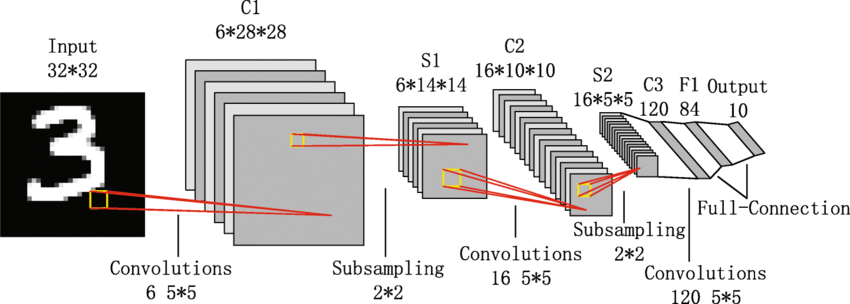
\includegraphics[width=0.8\textwidth,height=0.4\textheight,keepaspectratio]{images/cnn/lenet5.png}
\caption{LeNet-5 architecture.}
\end{figure}
{\small
\begin{itemize}
    \item LeNet-5 is a pioneering convolutional neural network (CNN) architecture developed by Yann LeCun and his collaborators in the late 1980s and early 1990s.
    \item It was primarily designed for handwritten digit recognition, specifically for the MNIST dataset.
    \item The architecture consists of two convolutional layers, followed by subsampling (pooling) layers, and then fully connected layers.
    \item It introduced key concepts such as convolutional layers, pooling layers, and the use of activation functions like sigmoid
\end{itemize}
}
\end{frame}

% AlexNet
\begin{frame}{AlexNet}
\begin{itemize}
    \item First big improvement in image classification.
    \item Made use of CNN, pooling, dropout, ReLU and training on GPUs.
    \item 5 convolutional layers, followed by max-pooling layers; with three fully connected layers at the end

\end{itemize}

\begin{figure}
\centering
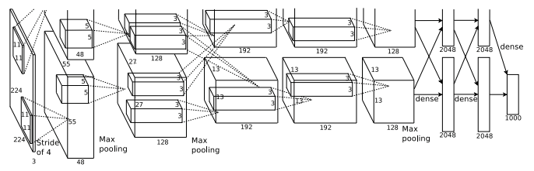
\includegraphics[width=1.0\textwidth,height=0.5\textheight,keepaspectratio]{images/cnn/alexnet.png}
\end{figure}
    
\end{frame}

% VGGNet
\begin{frame}{VGGNet}
\begin{itemize}
    \item \textbf{Improvement over AlexNet:} Uses a deeper network with small filters instead of a shallow network with larger filters.
    \item A stack of 3x3 conv layers (vs. 11x11 conv) has same receptive field, more non-linearities, fewer parameters and deeper network representation.
    \item Two variants: VGG16 or VGG19 conv layers plus 3 FC layers.
\end{itemize}

\begin{figure}
\centering
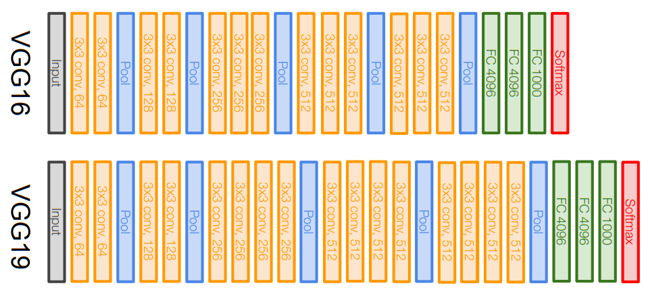
\includegraphics[width=1.0\textwidth,height=0.5\textheight,keepaspectratio]{images/cnn/VGG_16_19.png}
\end{figure}
    
\end{frame}

% InceptionNet
\begin{frame}[allowframebreaks]{InceptionNet}
    \begin{itemize}
        \item Going Deep: 22 layers
        \item Only 5 million parameters! (12× fewer than AlexNet, 27× fewer than VGGNet).
        \item Introduced efficient "Inception module"
        \item Introduced "bottleneck" layers that use 1x1 convolutions to reduce the number of channels and mix information across them.
    \end{itemize}

\begin{figure}
\centering
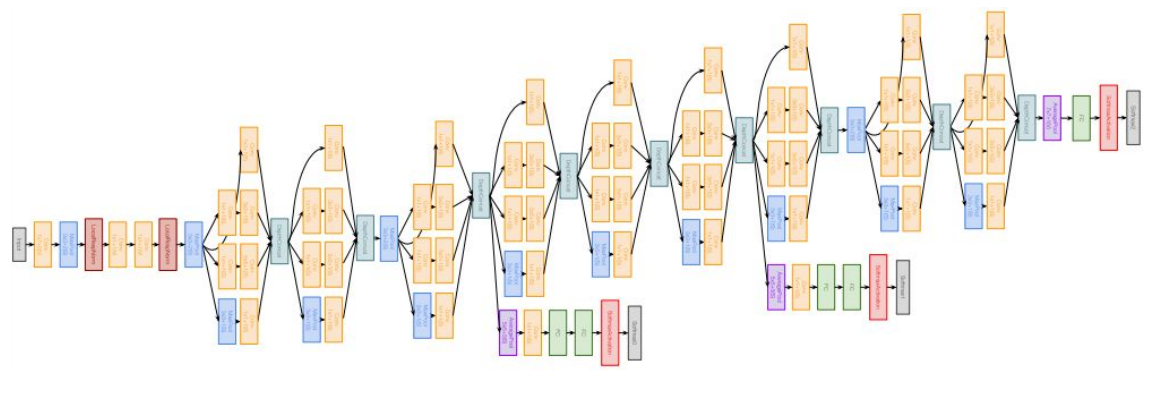
\includegraphics[width=1.0\textwidth,height=0.5\textheight,keepaspectratio]{images/cnn/inceptionnet_1.png}
\end{figure}

\framebreak

    \begin{itemize}
        \item \textbf{Inception module:} Uses multiple filter sizes (1×1, 3×3, 5×5), in parallel, to capture different features, then combines their outputs.

    \end{itemize}

\begin{figure}
\centering
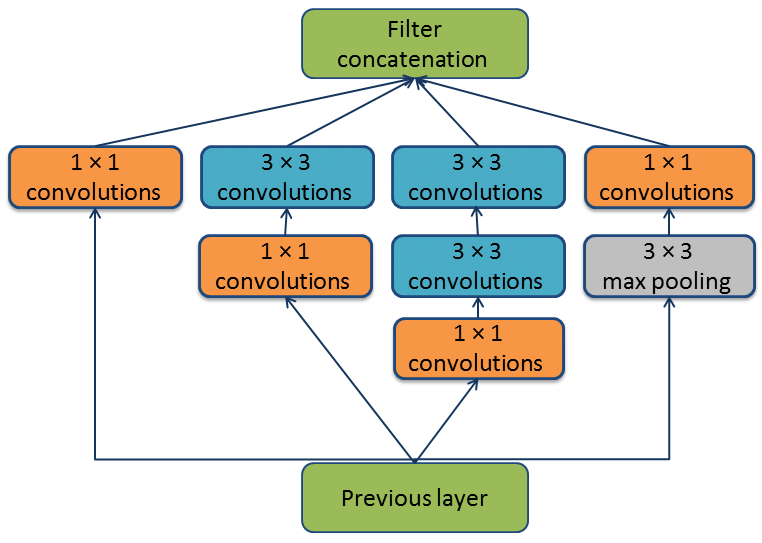
\includegraphics[width=1.0\textwidth,height=0.8\textheight,keepaspectratio]{images/cnn/inception_mod.png}
\end{figure}

\end{frame}

% ResNet
\begin{frame}{ResNet: Motivation}
\begin{itemize}
    \item \textbf{Problem:} Making networks deeper does not always improve accuracy.
    \item \textbf{Why?} In very deep networks, gradients become extremely small as they move backward through layers, making learning slow or stopping it altogether (\textbf{vanishing gradient problem}).
    \item \textbf{Solution:} Residual Network (ResNet) introduces \textbf{skip connections (residuals)}, allowing information to flow more easily.

\end{itemize}
\end{frame}

\begin{frame}{ResNet}
\begin{itemize}
    \item Very deep networks using residual connections
    \item 152-layer model for ImageNet
    \item Stacked Residual Blocks
    \item \textbf{Residual:} A shortcut connection that helps the network pass information through layers more easily.


\end{itemize}

\begin{figure}
\centering
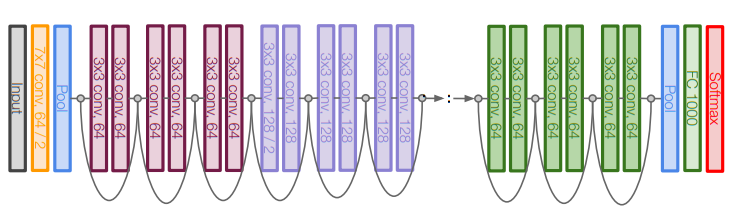
\includegraphics[width=1.0\textwidth,height=0.6\textheight,keepaspectratio]{images/cnn/resnet_1.png}
\end{figure}
\end{frame}

% EfficientNet
\begin{frame}{EfficientNet: Motivation}
\begin{itemize}
    \item \textbf{Problem:} To improve accuracy, we can:
    \begin{itemize}
        \item Increase the number of layers (\textbf{depth})
        \item Increase the number of neurons in each layer (\textbf{width})
        \item Use higher-resolution images (\textbf{resolution})
    \end{itemize}
    But finding the right balance of these three was largely based on trial and error.
    
    \item \textbf{Solution:} EfficientNet introduced a \textbf{compound scaling} method—a mathematical formula to systematically find the optimal balance among \textbf{depth}, \textbf{width}, and \textbf{resolution}.
\end{itemize}
\end{frame}

\begin{frame}{EfficientNet}

    \begin{figure}
        \centering
        % Replace with your own figure path
        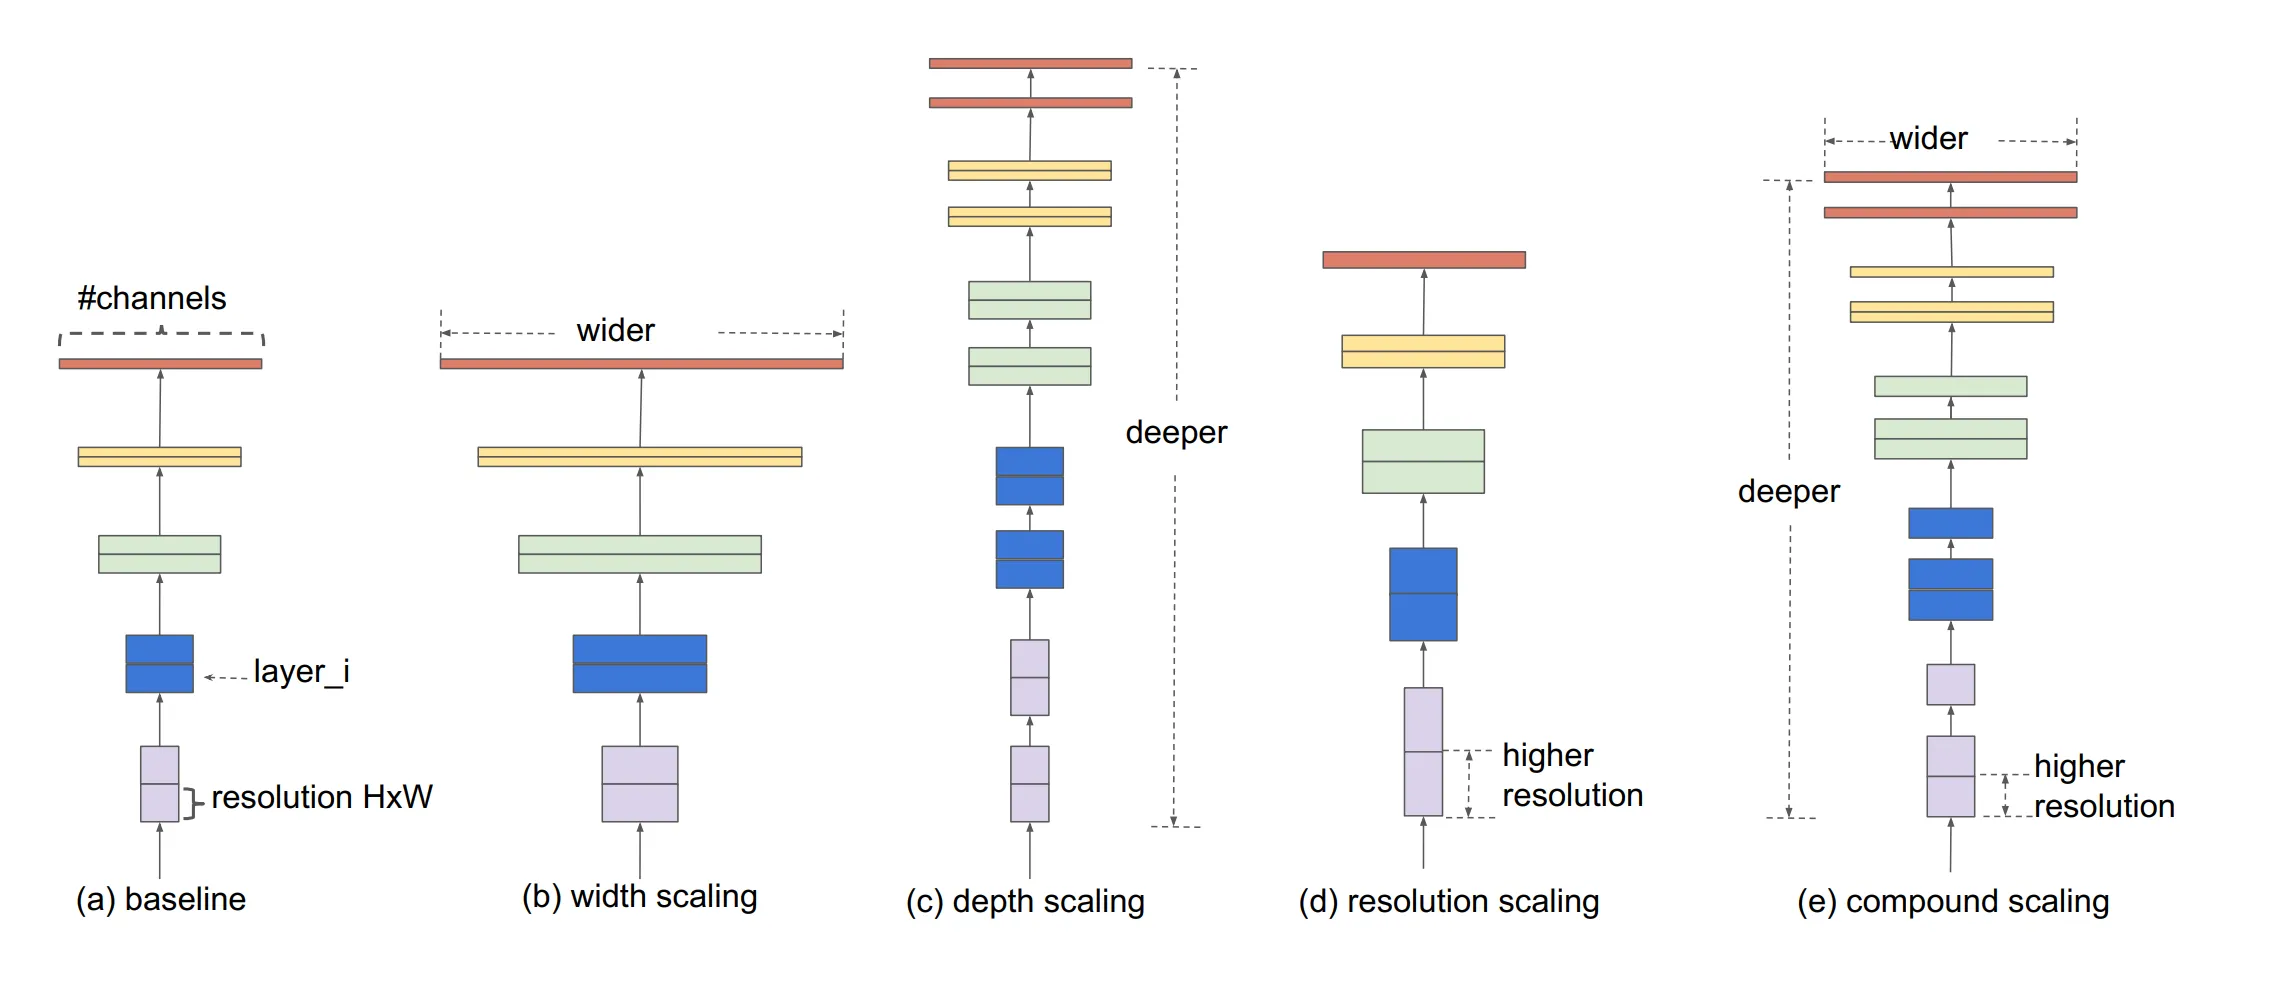
\includegraphics[width=\linewidth]{images/cnn/ENet_1.png}
        \caption{EfficientNet Scaling.}
    \end{figure}
\end{frame}


\begin{frame}{EfficientNet}
    \begin{itemize}
        \item \textbf{Compound Scaling} Uses a single \textbf{scaling coefficient} (\(\phi\)) to control:
        \begin{itemize}
        \item \textbf{Network Depth} (\(\alpha^\phi\)) → More layers
        \item \textbf{Network Width} (\(\beta^\phi\)) → More channels per layer
        \item \textbf{Input Resolution} (\(\gamma^\phi\)) → Larger input images
    \end{itemize}
        \item The goal: find \(\alpha, \beta, \gamma\) that balance accuracy \& efficiency, then scale up optimally by increasing the global coefficient \(\phi\).
    \end{itemize}

\end{frame}

\begin{frame}{EfficientNet}
\begin{itemize}
    \item EfficientNet optimizes depth, width, and resolution using this constraint:
    \[
    \alpha \cdot \beta^2 \cdot \gamma^2 \approx 2
    \]
    \item \textbf{Why this equation?}
    \begin{itemize}
        \item Increasing \textbf{depth} (\(\alpha\)) increases FLOPs \textbf{linearly}.
        \item Increasing \textbf{width} (\(\beta\)) increases FLOPs \textbf{quadratically} (\(\beta^2\)).
        \item Increasing \textbf{resolution} (\(\gamma\)) increases FLOPs \textbf{quadratically} (\(\gamma^2\)).
    \end{itemize}
    \item To double total FLOPs, the three factors must be balanced together.
\end{itemize}
\end{frame}



\begin{frame}{EfficientNet}
\begin{itemize}
    \item The authors of EfficientNet searched for the best scaling factors on a small baseline model.
    \item They found:
    \[
    \alpha = 1.2, \quad \beta = 1.1, \quad \gamma = 1.15
    \]
\end{itemize}
\end{frame}

\begin{frame}{EfficientNet Scaling: B0 to B7}
\begin{itemize}
    \item The EfficientNet family (B0 to B7) is generated using:
    \[
    \text{Depth} = 1.2^\phi, \quad
    \text{Width} = 1.1^\phi, \quad
    \text{Resolution} = 1.15^\phi
    \]
\end{itemize}

\begin{table}[]
    \centering
    \begin{tabular}{|c|c|c|c|}
        \hline
        \textbf{Model} & \(\phi\) & \textbf{Depth} (\(\alpha^\phi\)) & \textbf{Width} (\(\beta^\phi\)) \\ 
        \hline
        B0 & 0 & \(1.2^0 = 1.0\) & \(1.1^0 = 1.0\)  \\ 
        B1 & 1 & \(1.2^1 = 1.2\) & \(1.1^1 = 1.1\)  \\ 
        B2 & 2 & \(1.2^2 = 1.44\) & \(1.1^2 = 1.21\)  \\ 
        B3 & 3 & \(1.2^3 = 1.73\) & \(1.1^3 = 1.33\)  \\ 
        B4 & 4 & \(1.2^4 = 2.07\) & \(1.1^4 = 1.46\)  \\ 
        B5 & 5 & \(1.2^5 = 2.49\) & \(1.1^5 = 1.61\)  \\ 
        B6 & 6 & \(1.2^6 = 2.99\) & \(1.1^6 = 1.77\)  \\ 
        B7 & 7 & \(1.2^7 = 3.58\) & \(1.1^7 = 1.94\)  \\ 
        \hline
    \end{tabular}
    \caption{Scaling EfficientNet from B0 to B7}
\end{table}

\begin{itemize}
\item We multiply these scaling factors by the baseline EfficientNet-B0 values and round to the nearest integer to get the new depth, width, and resolution for each model.
\end{itemize}


\end{frame}


\begin{frame}{EfficientNet}

\begin{itemize}
    \item EfficientNet models achieve state-of-the-art accuracy with significantly fewer parameters and FLOPs.        \pause

    \item EfficientNet-B7 reaches 84.4\% Top-1 and 97.3\% Top-5 accuracy on ImageNet.
    \pause

    \item More efficient than previous CNN models---8.4x smaller and 6.1x faster than competitors.
\end{itemize}
\end{frame}


\begin{frame}{EfficientNet Performance}
\begin{figure}
\centering
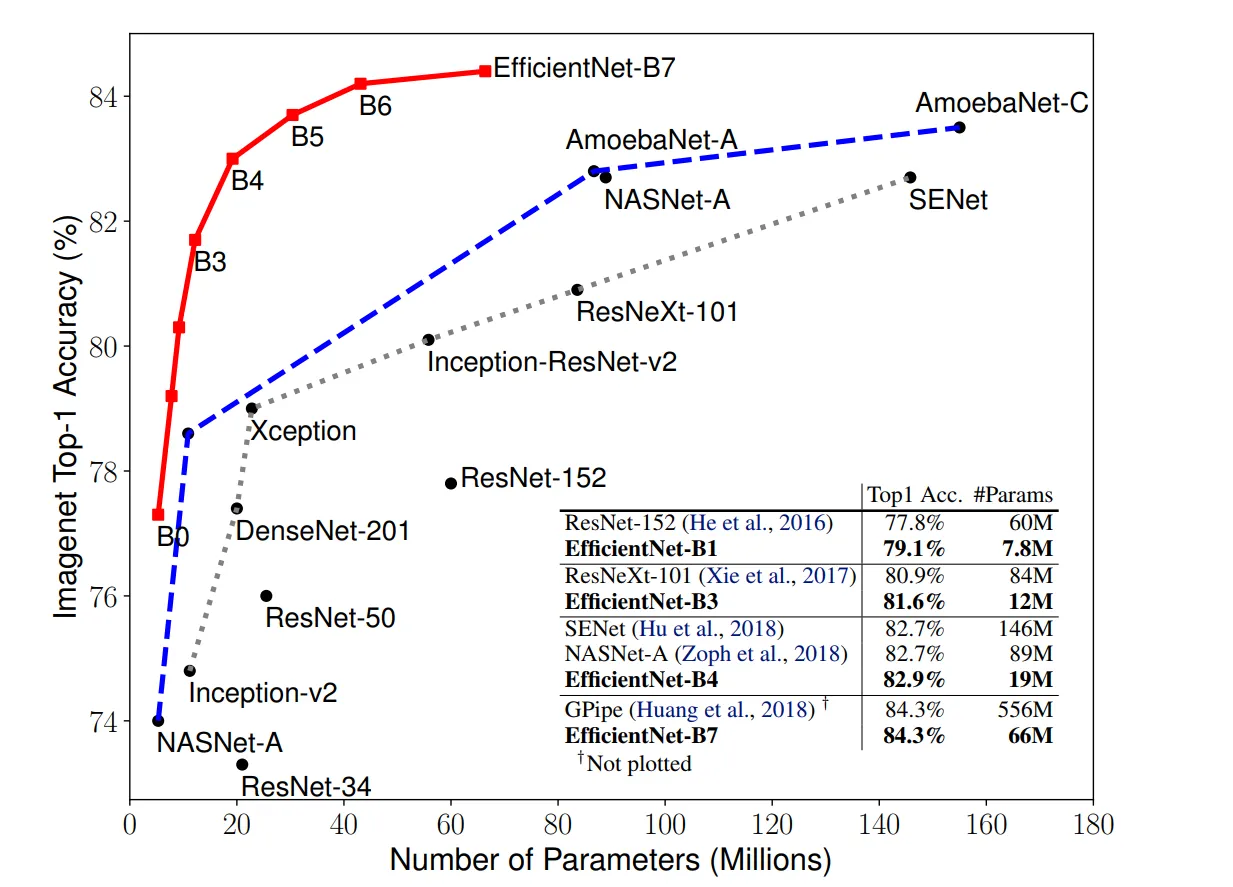
\includegraphics[width=\textwidth,height=.7\textheight,keepaspectratio]{images/cnn/ENet_2.png}
\caption{EfficientNet Performance on Imagenet.}
\end{figure}
\end{frame}

% MobileNet
\begin{frame}{Motivation for MobileNets}
\begin{itemize}
    \item \textbf{Why MobileNets?}
    \begin{itemize}
        \item Small-sized models are crucial for mobile and embedded devices.
        \item MobileNets reduce computational cost and memory usage while maintaining good accuracy.
    \end{itemize}
    \item \textbf{Key Idea:}
    \begin{itemize}
        \item Use \textbf{depthwise-separable convolutions} to significantly reduce computation compared to standard convolutions.
    \end{itemize}
\end{itemize}
\end{frame}

\begin{frame}{Computational Cost of Convolutions}
\begin{itemize}
    \item \textbf{Computational cost of standard convolution:}
    \[
    \text{Cost} = \text{\# filter params} \times \text{\# filter positions} \times \text{\# filters}
    \]
    \item Filters operate on all input channels, increasing computation significantly.
\end{itemize}
\begin{figure}
    \centering
    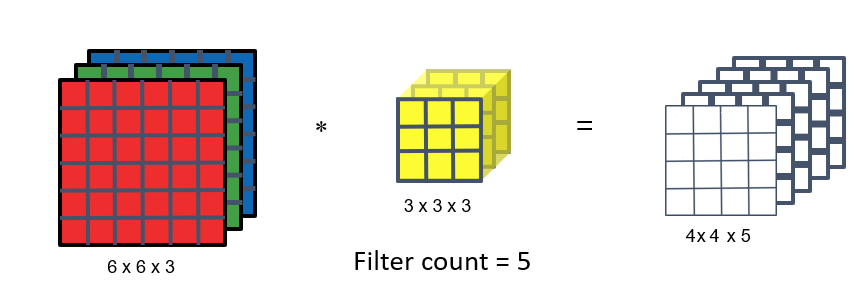
\includegraphics[width=0.8\linewidth]{images/cnn/NormalConv_MobileNet.png} 
\end{figure}
\end{frame}

\begin{frame}{Depthwise-Separable Convolutions}
\begin{itemize}
    \item Split standard convolution into two steps:
    \begin{itemize}
        \item \textbf{Depthwise Convolution:} Applies a single filter per input channel.
        \item \textbf{Pointwise Convolution:} Combines outputs from depthwise convolution.
    \end{itemize}
    \item \textbf{Key Benefit:} Reduces computational cost significantly compared to standard convolution.
\end{itemize}
\begin{figure}
    \centering
    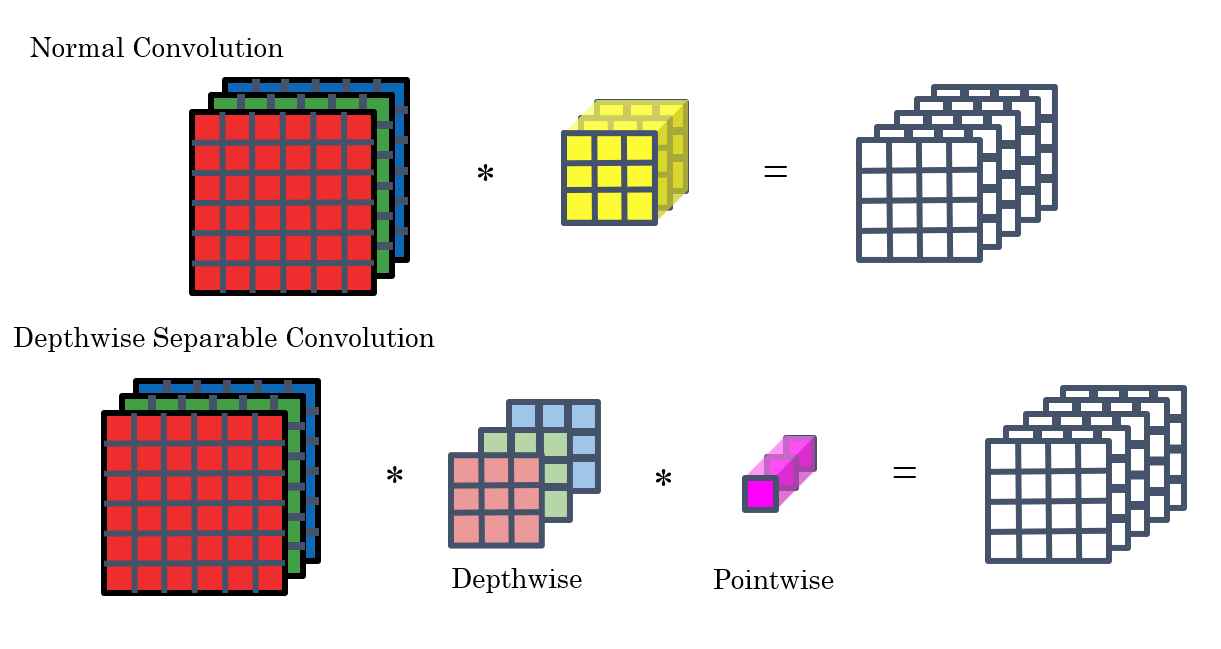
\includegraphics[width=0.8\linewidth]{images/cnn/Depth_vs_Normal_Conv.png} 
\end{figure}
\end{frame}

\begin{frame}{Depthwise Convolution}
\begin{itemize}
    \item Operates on each input channel separately.
\end{itemize}
\begin{figure}
    \centering
    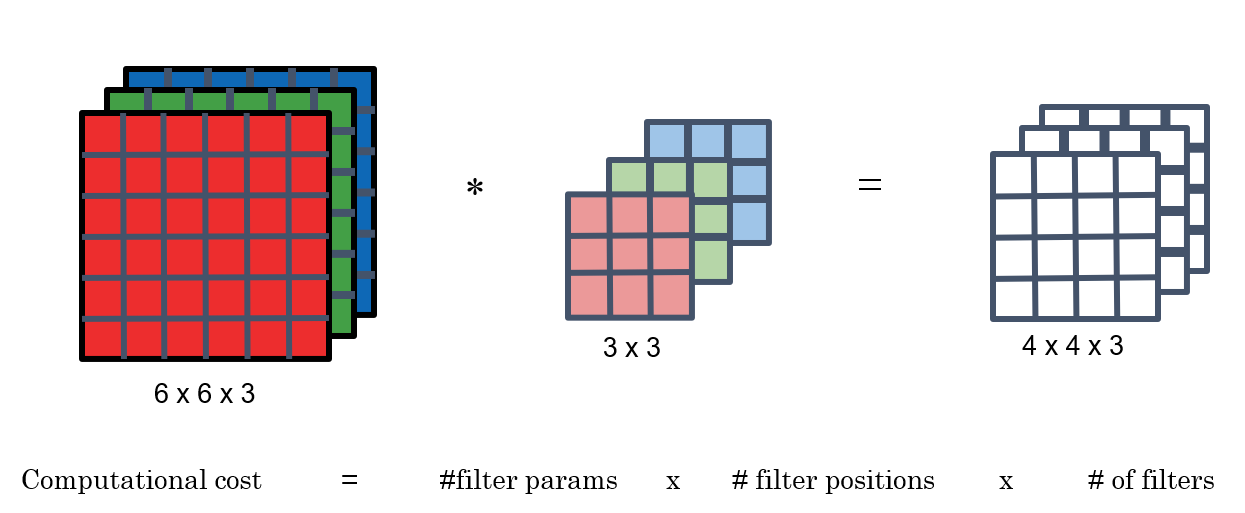
\includegraphics[width=0.8\linewidth]{images/cnn/Depthwise_conv.png}
\end{figure}
\end{frame}


\begin{frame}{Pointwise Convolution}
\begin{itemize}
    \item Combines outputs from depthwise convolution using \(1 \times 1\) convolutions (mixes channels).
\end{itemize}
\begin{figure}
    \centering
    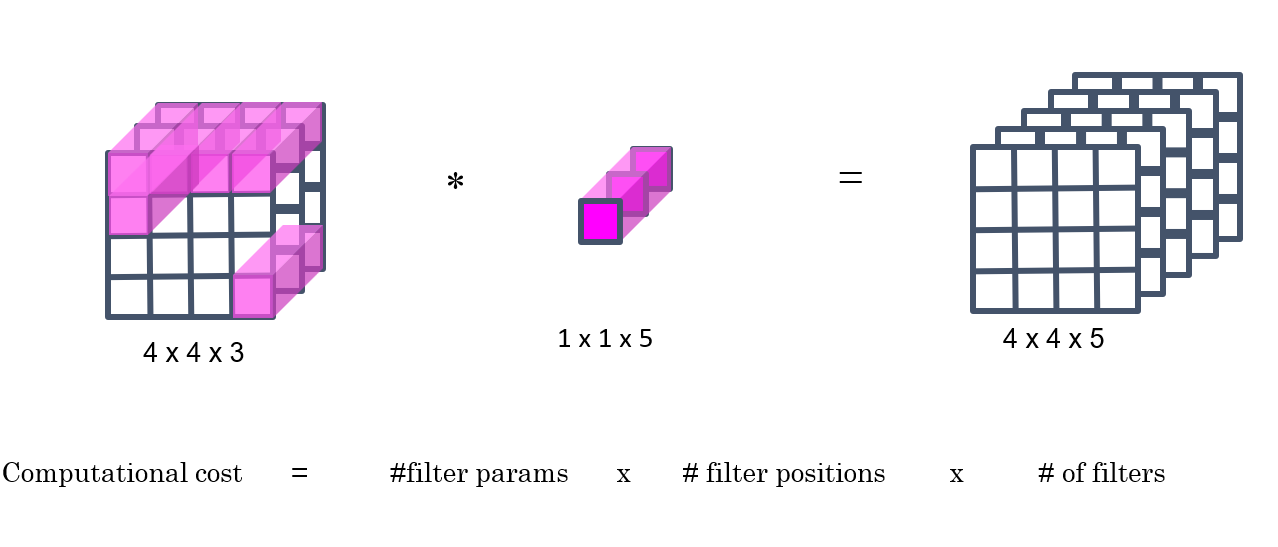
\includegraphics[width=0.8\linewidth]{images/cnn/PointWise_conv.png}
\end{figure}
\end{frame}

\begin{frame}{MobileNet Architectures}
\begin{itemize}
    \item \textbf{MobileNet v2:}
    \begin{itemize}
        \item Adds \textbf{residual connections}.
        \item Introduces:
        \begin{itemize}
            \item \textbf{Expansion step:} Expands input dimensions before depthwise convolution.
            \item \textbf{Projection step:} Reduces dimensions after processing.
        \end{itemize}
    \end{itemize}
\end{itemize}
\begin{figure}
    \centering
    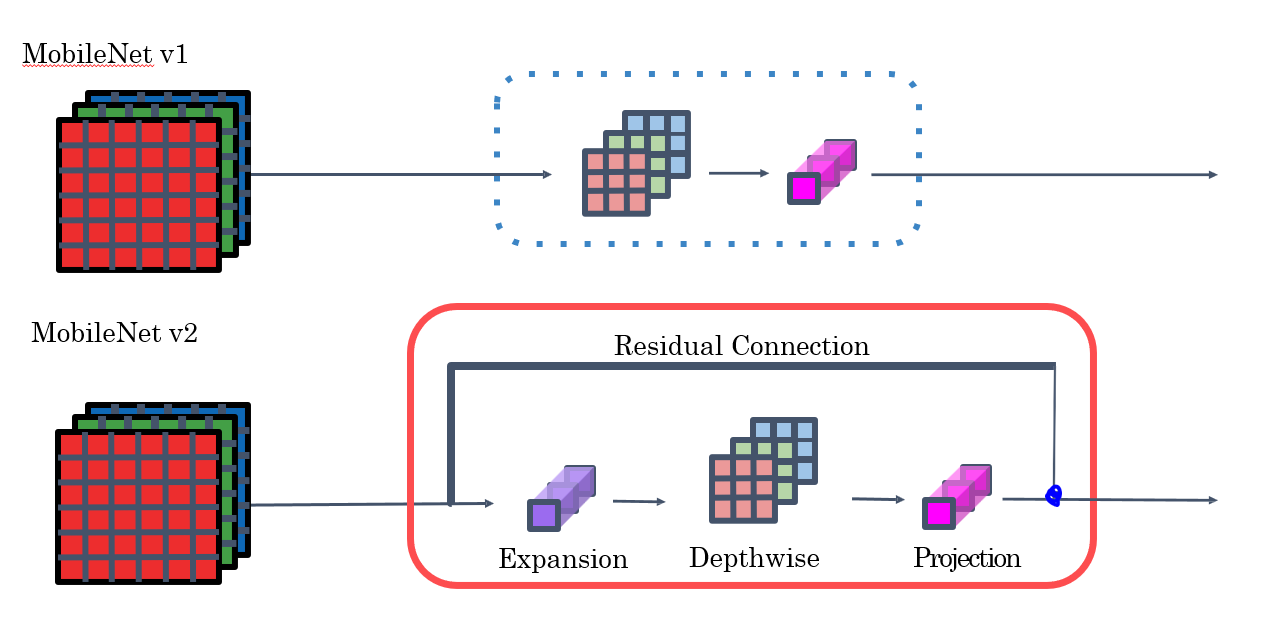
\includegraphics[width=0.8\textwidth,height=.7\textheight,keepaspectratio]{images/cnn/MobileNet_1_and_2.png} 
\end{figure}
\end{frame}

\section{Transfer Learning}
\begin{frame}{}
    \LARGE CNN: \textbf{Transfer Learning}
\end{frame}

\begin{frame}{What is Transfer Learning?}
    \begin{itemize}
        \item \textbf{Transfer Learning} is the process of reusing a model trained on one task (e.g., ImageNet classification) for a different but related task (e.g., medical image analysis).
        \item \textbf{Why use it?}
        \begin{itemize}
            \item Saves training time and computational resources.
            \item Achieves good performance with limited data.
        \end{itemize}
        \item \textbf{Types:}
        \begin{itemize}
            \item \textbf{Feature extraction:} Freeze convolutional layers and only train the final classifier.
            \item \textbf{Fine-tuning:} Unfreeze some or all layers and retrain on the new task.
        \end{itemize}
    \end{itemize}
\end{frame}

\begin{frame}{Transfer Learning Example}
    \begin{itemize}
        \item \textbf{Example:} Load a pretrained ResNet50 from PyTorch.
        \item Replace the last (classification) layer to match your number of classes.
        \item Optionally unfreeze the last few layers and retrain (fine-tuning).
    \end{itemize}
    \vspace{0.5cm}
    \textbf{Use cases:}
    \begin{itemize}
        \item Medical imaging
        \item Satellite imagery
        \item Small business datasets with limited data
    \end{itemize}
\end{frame}

\begin{frame}[fragile]{PyTorch Transfer Learning Code}
    \begin{lstlisting}[language=Python]
import torch
import torchvision.models as models
import torch.nn as nn

# Load pretrained ResNet50
model = models.resnet50(pretrained=True)

# Freeze all layers
for param in model.parameters():
    param.requires_grad = False

# Replace the final layer for 3 classes
num_ftrs = model.fc.in_features
model.fc = nn.Linear(num_ftrs, 3)

# Optionally unfreeze last few layers for fine-tuning
for param in list(model.parameters())[-10:]:
    param.requires_grad = True
    \end{lstlisting}
\end{frame}


\begin{frame}{Benefits of Transfer Learning}
    \begin{itemize}
        \item \textbf{Faster Training:} Pretrained models converge faster than training from scratch.
        \item \textbf{Better Performance:} Leverages learned features from large datasets.
        \item \textbf{Reduced Overfitting:} Especially useful when training data is limited.
        \item \textbf{Flexibility:} Can adapt to various tasks with minimal changes.
    \end{itemize}
    \vspace{0.5cm}
    \textbf{Considerations:}
    \begin{itemize}
        \item Ensure the pretrained model is suitable for your task.
        \item Fine-tuning requires careful selection of layers to unfreeze.
        \item Monitor for overfitting, especially with small datasets.
    \end{itemize}
\end{frame}

\begin{frame}{Putting it All Together}
    \begin{itemize}
        \item \textbf{Pick a solid architecture:} Start with proven models like ResNet, MobileNet, etc.
        \item \textbf{Use data augmentation:} Enrich your dataset with transformations to improve generalization.
        \item \textbf{Start with a pretrained model:} Leverage transfer learning for faster convergence and better performance.
        \item \textbf{Normalize activations:} Use Batch Normalization to stabilize and speed up training.
        \item \textbf{Regularize:} Apply Dropout and Early Stopping to prevent overfitting.
    \end{itemize}
\end{frame}
\begin{frame}[fragile, allowframebreaks]{CNN - Evaluation Metrics}
\begin{block}{Accuracy:}
    \begin{itemize}
        \item The ratio of correctly predicted instances to the total instances.
        \item It is a common metric for classification tasks.
        \item Formula: 
            \[
            \text{Accuracy} = \frac{\text{TP} + \text{TN}}{\text{TP} + \text{TN} + \text{FP} + \text{FN}}
            \]
        \item Where:
            \begin{itemize}
                \item TP: True Positives
                \item TN: True Negatives
                \item FP: False Positives
                \item FN: False Negatives
            \end{itemize}
        \item Limitations:
            \begin{itemize}
                \item It can be misleading in imbalanced datasets.
                \item It does not provide information about the types of errors made.
            \end{itemize}
    \end{itemize}
\end{block}
\framebreak
\begin{block}{Precision:}
    \begin{itemize}
        \item The ratio of correctly predicted positive instances to the total predicted positive instances.
        \item Formula: 
            \[
            \text{Precision} = \frac{\text{TP}}{\text{TP} + \text{FP}}
            \]
        \item It indicates how many of the predicted positive instances were actually positive.
        \item High precision means fewer false positives.
        \item Limitations:
            \begin{itemize}
                \item It does not consider false negatives.
                \item It can be misleading in imbalanced datasets.
            \end{itemize}
    \end{itemize}
\end{block}
\framebreak
\begin{block}{Recall:}
    \begin{itemize}
        \item The ratio of correctly predicted positive instances to the total actual positive instances.
        \item Formula: 
            \[
            \text{Recall} = \frac{\text{TP}}{\text{TP} + \text{FN}}
            \]
        \item It indicates how many of the actual positive instances were predicted correctly.
        \item High recall means fewer false negatives.
        \item Limitations:
            \begin{itemize}
                \item It does not consider false positives.
                \item It can be misleading in imbalanced datasets.
            \end{itemize}
    \end{itemize}
\end{block}
\framebreak
\begin{block}{F1 Score:}
    \begin{itemize}
        \item The harmonic mean of precision and recall.
        \item Formula: 
            \[
            \text{F1 Score} = 2 \cdot \frac{\text{Precision} \cdot \text{Recall}}{\text{Precision} + \text{Recall}}
            \]
        \item It provides a balance between precision and recall.
        \item Useful for imbalanced datasets where one class is more important than the other.
        \item Limitations:
            \begin{itemize}
                \item It can be misleading if the precision and recall are very different.
                \item It does not provide information about the types of errors made.
            \end{itemize}
    \end{itemize}
\end{block}
\framebreak
\begin{block}{Confusion Matrix:}
    \begin{itemize}
        \item A table that summarizes the performance of a classification model.
        \item It shows the true positive, true negative, false positive, and false negative counts.
        \item It provides a detailed breakdown of the model's performance.
        \item Useful for understanding the types of errors made by the model.
        \item Can be used to calculate other metrics like accuracy, precision, recall, and F1 score.
        \item Example:
            \[
            \begin{array}{|c|c|c|}
            \hline
            & \text{Predicted Positive} & \text{Predicted Negative} \\
            \hline
            \text{Actual Positive} & \text{TP} & \text{FN} \\
            \hline
            \text{Actual Negative} & \text{FP} & \text{TN} \\
            \hline
            \end{array}
            \]
        \item Where:
            \begin{itemize}
                \item TP: True Positives
                \item TN: True Negatives
                \item FP: False Positives
                \item FN: False Negatives
            \end{itemize}
    \end{itemize}
\end{block}
\framebreak

\begin{block}{mAP:}
    \begin{itemize}
        \item mAP is calculated by averaging the average precision (AP) across all classes.
        \item AP is calculated by plotting the precision-recall curve and computing the area under the curve.
        \item mAP is particularly useful for evaluating models on datasets with multiple classes.
        \item It provides a comprehensive measure of the model's performance across all classes.
        \item Example:
            \[
            \text{mAP} = \frac{1}{N} \sum_{i=1}^{N} \text{AP}_i
            \]
            \item Where:
                \begin{itemize}
                    \item \(N\) is the number of classes.
                    \item \(\text{AP}_i\) is the average precision for class \(i\).
                \end{itemize}
        \item mAP can be calculated at different IoU thresholds (e.g., 0.5, 0.75) to evaluate the model's performance at different levels of overlap.
    \end{itemize}
\end{block}
\framebreak

\begin{lstlisting}[language=Python, caption={Code snippet (PyTorch)}, basicstyle=\ttfamily\footnotesize]
from torcheval.metrics.functional import multiclass_precision, multiclass_recall, multiclass_f1_score

p = multiclass_precision(preds, labels)
r = multiclass_recall(preds, labels)
f1= multiclass_f1_score(preds, labels)
\end{lstlisting}
\end{frame} 
\begin{frame}[fragile, allowframebreaks]{CNN - Further Reading}
\begin{block}{Books:}
    \begin{itemize}
    \item \textbf{Deep Learning} by Ian Goodfellow, Yoshua Bengio, and Aaron Courville \vspace{0.5em}
    \item \textbf{Hands-On Machine Learning with Scikit-Learn, Keras, and TensorFlow} by Aurélien Géron \vspace{0.5em}
    \item \textbf{Pattern Recognition and Machine Learning} by Christopher Bishop \vspace{0.5em}
    \item \textbf{Deep Learning for Computer Vision with Python} by Adrian Rosebrock
    \end{itemize}
\end{block}
\framebreak
\begin{block}{Online Courses:}
    \begin{itemize}
        \item \textbf{Deep Learning Specialization} by Andrew Ng (Coursera) \vspace{0.5em}
        \item \textbf{Convolutional Neural Networks for Visual Recognition} by Fei-Fei Li (Stanford University) \vspace{0.5em}
        \item \textbf{Practical Deep Learning for Coders} by Jeremy Howard (fast.ai) \vspace{0.5em}
        \item \textbf{Deep Learning with PyTorch} by Facebook AI Research \vspace{0.5em}
    \end{itemize}
\end{block}
\framebreak
\begin{block}{Research Papers:}
    \begin{itemize}
        \item \textbf{ImageNet Classification with Deep Convolutional Neural Networks} by Alex Krizhevsky, Ilya Sutskever, and Geoffrey Hinton \vspace{0.5em}
        \item \textbf{Very Deep Convolutional Networks for Large-Scale Image Recognition} by K. Simonyan and A. Zisserman \vspace{0.5em}
        \item \textbf{Deep Residual Learning for Image Recognition} by Kaiming He et al. \vspace{0.5em}
        \item \textbf{Densely Connected Convolutional Networks} by Gao Huang et al. \vspace{0.5em}
    \end{itemize}
\end{block}
\framebreak
\begin{block}{Websites and Blogs:}
    \begin{itemize}
        \item \textbf{Towards Data Science} (Medium)
        \item \textbf{Distill.pub} (Research and visualization)
        \item \textbf{Kaggle} (Datasets and competitions)
        \item \textbf{Papers with Code} (Research papers with code implementations)
    \end{itemize}
\end{block}
\framebreak
\begin{block}{YouTube Channels:}
    \begin{itemize}
        \item \textbf{3Blue1Brown} (Mathematics and deep learning)
        \item \textbf{Two Minute Papers} (Research summaries)
        \item \textbf{Sentdex} (Python programming and machine learning)
        \item \textbf{StatQuest with Josh Starmer} (Statistics and machine learning)
    \end{itemize}
\end{block}
\framebreak
\begin{block}{GitHub Repositories:}
    \begin{itemize}
        \item \textbf{TensorFlow Models} (TensorFlow implementations)
        \item \textbf{PyTorch Examples} (PyTorch implementations)
        \item \textbf{fastai} (High-level library for deep learning)
        \item \textbf{Keras} (High-level neural networks API)
    \end{itemize}
\end{block}
\framebreak
\begin{block}{Conferences:}
    \begin{itemize}
        \item \textbf{NeurIPS} (Neural Information Processing Systems)
        \item \textbf{CVPR} (Computer Vision and Pattern Recognition)
        \item \textbf{ICML} (International Conference on Machine Learning)
        \item \textbf{ICLR} (International Conference on Learning Representations)
    \end{itemize}
\end{block}
\end{frame}

\begin{frame}[plain]
  \frametitle{Credits}
  \begin{center}
    \textbf{Credits} \\[1.5em]

    \Large Dr. Prashant Aparajeya \\[0.5em]
    {\normalsize Computer Vision Scientist | Director(AISimply Ltd)} \\[0.5em]
    \footnotesize \href{mailto:p.aparajeya@aisimply.uk}{p.aparajeya@aisimply.uk} \\[2em]

    {\footnotesize This project benefited from external collaboration, and we acknowledge their contribution with gratitude.}
  \end{center}
\end{frame}


\end{document} 